\documentclass[twoside,openright,a4paper,papersize,uplatex,dvipdfmx]{jsbook}
% uplatex オプションを指定し、ユニコード対応に。ただだし、uplatex でコンパイルすること。

% 修論本体と表紙で共通で必要となる設定
% jsbookで余白が広すぎるのを直す
% 参照 https://oku.edu.mie-u.ac.jp/~okumura/jsclasses/
\setlength{\textwidth}{\fullwidth}
\setlength{\evensidemargin}{\oddsidemargin}
\addtolength{\textwidth}{-5truemm}
\addtolength{\oddsidemargin}{5truemm}

% 同梱の ISEE 用の表紙テンプレ
\usepackage{thesis_cover}

% OTF フォントを使えるようにし、複数のウェイトも使用可能にする。
% これがないと、Mac のヒラギノ環境で使われる角ゴが太すぎてみっともない。
\usepackage[deluxe]{otf}
% OT1→T1に変更し、ウムラウトなどを PDF 出力で合成文字ではなくす
\usepackage[T1]{fontenc}
% uplatex の場合に必要な処理 
\usepackage[utf8]{inputenc} % エンコーディングが UTF8 であることを明示する。
\usepackage[prefernoncjk]{pxcjkcat} % アクセントつきラテン文字を欧文扱いにする
% Helvetica と Times を sf と rm のそれぞれで使う。
% default だとバランスが悪いので、日本語に合わせて文字の大きさを調整する。
\usepackage[scaled=1.05,helvratio=0.95]{newtxtext}
% 色
\usepackage[dvipdfmx]{color}
% 行番号を表示する。
\usepackage{lineno}

% latexdiff
% 実際の修論には入れる必要なし
%DIF PREAMBLE EXTENSION ADDED BY LATEXDIFF
%DIF UNDERLINE PREAMBLE %DIF PREAMBLE
\RequirePackage[normalem]{ulem} %DIF PREAMBLE
\RequirePackage{color}\definecolor{RED}{rgb}{1,0,0}\definecolor{BLUE}{rgb}{0,0,1} %DIF PREAMBLE
\providecommand{\DIFadd}[1]{{\protect\color{blue}\uwave{#1}}} %DIF PREAMBLE
\providecommand{\DIFdel}[1]{{\protect\color{red}\sout{#1}}}                      %DIF PREAMBLE
%DIF SAFE PREAMBLE %DIF PREAMBLE
\providecommand{\DIFaddbegin}{} %DIF PREAMBLE
\providecommand{\DIFaddend}{} %DIF PREAMBLE
\providecommand{\DIFdelbegin}{} %DIF PREAMBLE
\providecommand{\DIFdelend}{} %DIF PREAMBLE
%DIF FLOATSAFE PREAMBLE %DIF PREAMBLE
\providecommand{\DIFaddFL}[1]{\DIFadd{#1}} %DIF PREAMBLE
\providecommand{\DIFdelFL}[1]{\DIFdel{#1}} %DIF PREAMBLE
\providecommand{\DIFaddbeginFL}{} %DIF PREAMBLE
\providecommand{\DIFaddendFL}{} %DIF PREAMBLE
\providecommand{\DIFdelbeginFL}{} %DIF PREAMBLE
\providecommand{\DIFdelendFL}{} %DIF PREAMBLE
%DIF END PREAMBLE EXTENSION ADDED BY LATEXDIFF


%% 以下追加したpackage
% 画像の取り扱いに必要
\usepackage{graphicx}
% 数式の機能を拡張
\usepackage{amsmath}
\usepackage{bm}
\usepackage{upgreek}
\usepackage{newtxmath,newtxtext}
% コードを表示
\usepackage{listings}
\lstset{
    %プログラム言語(複数の言語に対応,C,C++も可)
    language = Python,
    %背景色と透過度
    backgroundcolor={\color[gray]{.98}},
    %枠外に行った時の自動改行
    breaklines = true,
    %自動改行後のインデント量(デフォルトでは20[pt])	
    breakindent = 10pt,
    %標準の書体
    basicstyle = \ttfamily\scriptsize,
    %コメントの書体
    commentstyle = {\itshape \color[cmyk]{1,0.4,1,0}},
    %関数名等の色の設定
    classoffset = 0,
    %キーワード(int, ifなど)の書体
    keywordstyle = {\bfseries \color[cmyk]{0,1,0,0}},
    %表示する文字の書体
    stringstyle = {\ttfamily \color[rgb]{0,0,1}},
    %枠 "t"は上に線を記載, "T"は上に二重線を記載
    %他オプション:leftline,topline,bottomline,lines,single,shadowbox
    frame = tbrl,
    %frameまでの間隔(行番号とプログラムの間)
    framesep = 5pt,
    %行番号の位置
    numbers = left,
    %行番号の間隔
    stepnumber = 1,
    %行番号の書体
    numberstyle = \tiny,
    %タブの大きさ
    tabsize = 4,
    %キャプションの場所("tb"ならば上下両方に記載)
    captionpos = t
}
% 複数引用
\usepackage{cite}
%\usepackage{natbib}
% 複数図を並べる時のcaption
\usepackage{subcaption}
\usepackage{here}
% 表関連
\usepackage{booktabs}
% 表でセルを複数列で結合する
\usepackage{multicol}
\usepackage{multirow}
% PDF 内で外部リンクや文書内リンクを生成したい場合に使う(好みによる)
\usepackage[dvipdfmx, hidelinks]{hyperref}
\usepackage{url}
% 複数行コメント
\usepackage{comment}
% 番号付き箇条書きのオプション利用
\usepackage{enumerate}
% renewcommandなどはここに
\usepackage{mymacros}
% 目次でsubsectionまで表示
\setcounter{tocdepth}{2}



% 画像の取り扱いに必要
\usepackage{graphicx}

% 表でセルを複数列で結合する
\usepackage{multicol}

% 数式の機能を拡張
\usepackage{amsmath}

% citep や citet を有効にする
\usepackage{natbib}

% (Okumura, 2009) などを (Okumura 2009) とする
% 日本語文章で全角丸括弧の表示にし、かつ \inhibitglue で役物同士の字間を適切にする。
% https://oku.edu.mie-u.ac.jp/tex/mod/forum/discuss.php?d=2349
\setcitestyle{aysep={},notesep={},open={\inhibitglue(},close={)\inhibitglue}}

% subfigure 環境で、(a)、(b) などの番号を左上に表示する。宇宙系の分野ではこれが一般的なはず。
% \usepackage[nooneline]{subfigure}
\usepackage{subcaption}
\usepackage{here}

% 表関連
\usepackage{booktabs}

% 行番号を表示する。添削時のみに使い、事務提出版ではコメントアウトする
%\usepackage{lineno}
%\linenumbers

% PDF 内で外部リンクや文書内リンクを生成したい場合に使う(好みによる)
\usepackage[dvipdfmx, hidelinks]{hyperref}

% newcommand を使うことで、繰り返し使う長ったらしい入力を簡単にすることができる
\makeatletter
\newcommand{\ion}[2]{#1$\;${\small\rmfamily\@Roman{#2}}\relax}%
\makeatother
\newcommand{\HI}{\mbox{\ion{H}{1}}} % 中性原子ガス(HI 領域)の例
\newcommand{\bs}{\symbol{92}} % backslash
\newcommand{\red}[1]{\textcolor{red}{#1}}


% renewcommandなどはここに
\usepackage{mymacro}
% 目次でsubsectionまで表示
\setcounter{tocdepth}{2}

% 氏名などの情報が入っているファイル。各自で編集。
\title{深層学習による消化管腫瘍検出 \\ 〜3次元病理画像解析〜} % 論文題目
\date{2019年1月31日} % 日付(入れたくなければ空欄)
\heisei{31} % 年度
\StudentIdNumber{37-176484} % 学籍番号
\author{松崎  博貴} % 氏名
\seifuku{} % 正本か副本か(このファイルでは変更する必要なし)
% \labname{宇宙線物理学研究室} %
\supervisor{小野寺宏 特任教授} % 指導教員
\cosupervisor{染谷隆夫 教授} % 副指導教員


\begin{document}
% 式番号,図番号,表番号を章ごとの連番にする
\numberwithin{equation}{chapter}
\numberwithin{figure}{chapter}
\numberwithin{table}{chapter}


\frontmatter

\maketitle

% これを入れることでページ番号が表示されない。
\thispagestyle{empty}

% abstract 環境は jsbook では「概要」と表示してくれないため、手動で表示させる。
% 参照 http://oku.edu.mie-u.ac.jp/tex/mod/forum/discuss.php?d=2121
\begin{center}
  {\large \sf 概要}
\end{center}

近年になって医療データが蓄積されるシステムができてきいる。医療画像をコンピューター上に取り込むようになってから、自動で解析するシステムを構築してきた。今までは、専門医が診断を行う場合は、判断が主観的であること、ミスをする可能性があること、専門化同士でも意見が異なること、実際の臨床現場で医師はたくさんの画像を処理しなくてはいけないので、1枚にかけられる時間が限られていることから、機械による診断支援システムが必要とされている。既存の機械によるルールベースによるシステムでは解析ルール人にバイアスがかかっているということや、画像認識の著しい精度向上があるディープラーニングを利用した方法によって解析する方法に注目されている。またコンピュータの計算性能と、ビッグデータである医療画像を処理する能力が向上した背景と重なって、現在は機械学習による医療画像解析の研究が盛り上がりを見せている。

\tableofcontents
\listoffigures
\listoftables

\mainmatter

% include を使うことで、別ファイルに分割することができます。
\chapter{序論}
\label{chap_intro}
\section{けんきゆうはいけい}
胃がんは、日本でもっとも罹患数が多いがんであり、年間13万人が罹患し5万人が亡くなっている.内視鏡の生検は食道,大腸,小腸,胃などを鉗子で2mm角の立方体程度の大きさで抜き出し,染色したものを2,3断面にカットしてから病理診断医が顕微鏡で観察,診断している.
断面のみの観察では内部に腫瘍がある場合に見落としてしまうリスクがあるため,本研究では組織透明化技術を用いて検体を丸ごと観察できるようにした。病理医が全てを診断するには負担が大きいことと病変の見落としリスクがあること,経験を詰んだ医師でも判断の難しい病変を見つけることが求められている。

内視鏡で見つけた病変が、腫瘍か非腫瘍かを判別したり、その悪性度を判定することは生検を観察する必要がある.内視鏡検査の専門医のマンパワーが不足している.現在の日本の病理の専門医は2259名で,その人数に対して標本 500万件を年間で処理している現状である.

また癌検診では担当医が判定して専門医がダブルチェックをしているが,AIがスクリーニングを行って専門医の確認が必要な症例を絞り込む.専門医の判定は主観的であることや,専門医ごとにも判断基準がことなることが課題になる.

\begin{figure}[H]
	\centering
	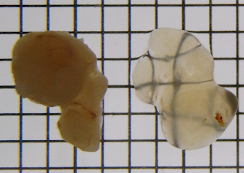
\includegraphics[width=0.7\linewidth]{fig/chapter1/lucid}
	\caption{transparent specimen}
	\label{fig:lucid}
\end{figure}

\begin{figure}[H]
	\centering
	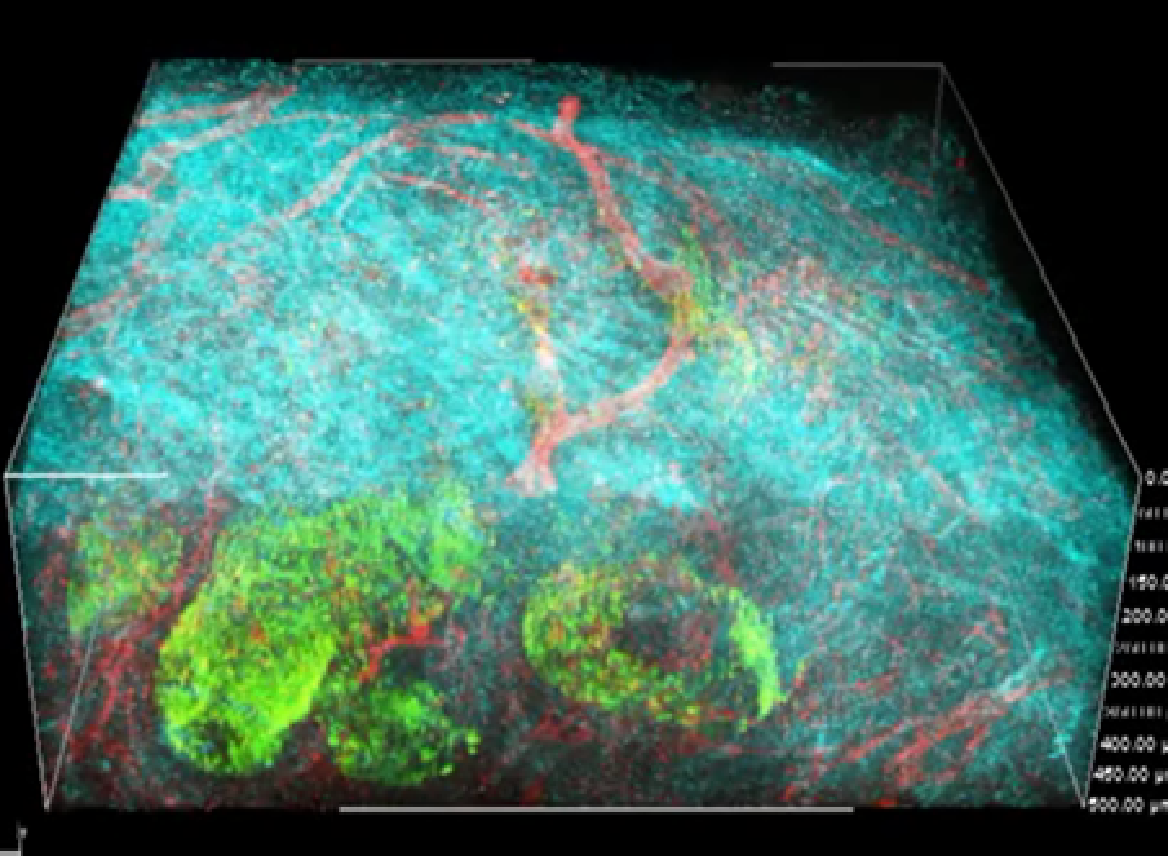
\includegraphics[width=0.7\linewidth]{fig/chapter1/microscope}
	\caption{microscope}
	\label{fig:microscope}
\end{figure}

\section{ほんけんきゆうのもくてき}
本研究の目的は内視鏡生検を透明にして深層学習を利用して癌を見落とさない診断方法を開発することである.組織透明化技術LUCIDを用いて検体を丸ごと透明化し,レーザー顕微鏡で観察することで,顕微鏡の解像度で検体の内部まで3次元情報として解析することができる.

\begin{figure}[H]
	\centering
	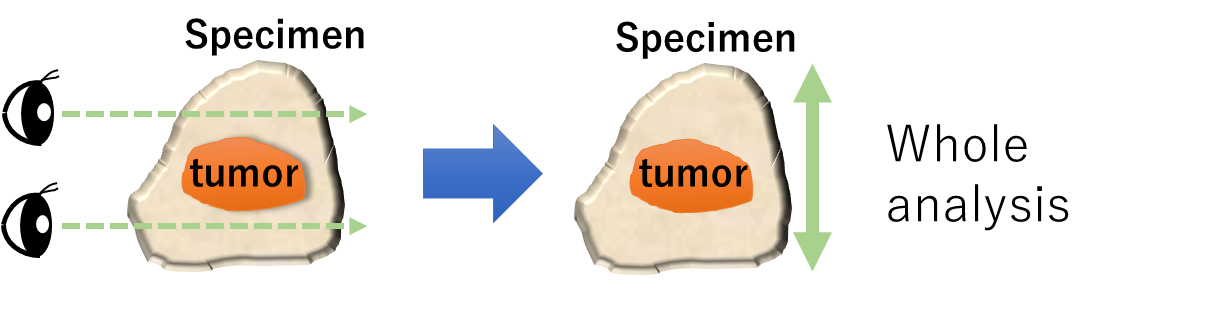
\includegraphics[width=0.7\linewidth]{fig/chapter1/whole_image_analysis}
	\caption{whole image analysis}
	\label{fig:wholeimageanalysis}
\end{figure}


透明化されたサンプルをレーザー顕微鏡で撮影すると,従来のカットする手法に換算して1000カットに相当するため,得られる顕微鏡撮影像が従来の2,3カットに対して数100倍となるので,専門医が診断をするには負担が大きくなってしまう.したがって,人工知能(Artificial Intelligence: AI)が3次元画像を解析して病変を検知し,専門医に提示することで病変の見落としリスクがゼロになる診断支援システムを開発することが本研究の目的である.

AIを用いた内視鏡の診断支援は生検ではなくて、内視鏡カメラの画像解析を行う事例がある。国立がん研究センターとNECが共同で開発したシステムがある。しかし、診断を確定するには生検が必須であり、生検の病理診断にマンパワーが必要になっている。生検のAIによる診断アルゴリズム開発の先行研究としては、胃がん、肺がんや乳がん、骨髄などの生検をディープラーニングで境界認識するものががあり、90\%程度の正解率を出して、専門医と同程度の精度がすでに達成されているものもあるがデータセットとして提供されているのは単純の形状のものが多い。本研究では生検の3次元画像を解析することで2次元画像では判断の難しいものを3次元特有の情報を用いることで判定精度を上げ、
機械学習を行うためには教師データを用意する必要があるが、医療データはアノテーションされていないことが多い。3次元画像を解析する先行研究としては、CTやMRI画像が上げられる。CTやMRIの場合は画像の分解能が顕微鏡像よりも低く、深さ方向にも30程度である。本研究は透明化処理した生検を蛍光顕微鏡で撮影するため分解能が高く、深さ方向にも400~700枚が撮影することができる。このためディープラーニングで解析するときに計算のメモリに乗らないという問題が生じるため解析手法を工夫して計算量がなるべく減るようにしなければいけない。今回は時系列処理で使われる手法と画像処理の手法を組み合わせて用いることで、大きな画像サイズでも解析することができるようにした。


深層学習で解析を行う場合はデータを大量に準備する必要がある.今回のように,新しい撮影手法であったり,希少な病気であったりすると医療データを数多く集められないことがある.さらに画像データだけでなく,その画像に教師ラベルを貼る(アノテーション)必要がある.画像と,その教師ラベルのセットを数万枚と集めることができたら高い精度が出るという報告が多くあるが,少ない教師データで識別精度を上げることは深層学習において困難とされている.教師データの作成が困難であるだけでなく,少量データである場合は,その教師データが医師によってばらつきがある場合は,教師データを作成した医師の判断が大きく反映されてしまい,必ずしも真であると断言することができなくなってしまう.これらの課題があるため医療画像における深層学習を用いた診断システムは,大量にデータを用意するまでの時間や人的コストを大きく払うことになっているのが現状である.

本研究でこの課題に取り組んだ.教師ラベルを必要とせず,画像の構造的な特徴のパターンを学ぶ,教師なし学習の手法と,これまでの教師ラベルを使った学習とを組み合わせた,半(弱)教師あり学習を行った.構造的なパターンは3次元画像であることを活用し,教師なし学習については,病理画像が正常から異常になる過程には連続的な性質があることを活用して正常と異常の分布が作れるようにした.


最後にこの深層学習による腫瘍の検出結果を医師が診断する際のサポートになるように可視化する.深層学習は,よく判断の理由が分からないためブラックボックスと呼ばれ,信頼性が求められる場面では利用に対して不安視されることがある.そのため腫瘍と正常の診断の判断の理由が可視化して,どの部分に注目しているかを医師に見せる.医師の負担を減らすためのスクリーニングとして利用するために,明らかに正常のものと,腫瘍かもしれない領域とを区別して,腫瘍かもしれない部分を医師に提示する.3次元画像であるから医師が診断するには,全ての断面を確認することは現実的に不可能である.腫瘍を見落とさないように,深層学習によって,腫瘍がある確率の高い断面を提示して診断支援を行う.

\chapter{深層学習による病理画像の診断支援}
\label{chap_review}

病理画像をデジタルで保存することが始まったのは数十年前になる.これによって遠隔地でも診断することができるようになったり,情報を共有することができるようになり,複数の医師で診断しミスを防止するセカンド・オピニオンが容易になった.計算機科学の分野の側面ではデータを収集することができるようになり,研究が盛んに行われることになった.その後は,様々な病理データでより改良されたアルゴリズムの提案が行われている.

細胞組織の形態を観察するための病理染色ではヘマトキシリン・エオジン染色(HE染色)が一般的に用いられる.細胞核を青紫色に染色し,細胞質をピンク色に染色する.正常から異常に変化していくと,細胞核が過度に増殖したり,細胞質の形が崩れたりすることで,その特徴を機械学習によって精度よく検出するための研究が行われている.

これまでは,核の形やテキスチャーからパターンマッチングなどの画像処理によって腫瘍を検出する研究されてきたが,近年になって画像処理に大きなブレークスルーが起きたことをきっかけに,新しい手法で解析するようになってきた.そのブレークスルーがディープラーニングである.

\section{ニューラルネットワーク}\label{sec:NeuralNetwork}
人間の脳にはニューロンと呼ばれる神経細胞が1000億個以上あり,それぞれが複数のニューロンが電気信号によって情報を伝達している.また脳にはシナプスという場所があり,ここで電気信号を細胞体へ受け渡す.細胞体はある閾値以上の電気信号がきた場合に他のニューロンへ電気信号を伝播させる(これを発火と呼ぶ).このようなニューロンとシナプスで行われる演算を模倣したアルゴリズムを作ることができれば,人間のような思考や認識をコンピュータを使って再現できると考えた.そのアルゴリズムがニューラルネットワーク(Neural Network: NN)である.

\subsection{多層パーセプトロン}
ニューラルネットワークは入力層,出力層,隠れ層から構成され,層と層の間にはニューロン同士のつながりの強さを示す重みがある.非線形問題を扱うために1986年Rumelhartによって考案されたのが,パーセプトロンを複数つなぎ合わせ入力と出力以外に隠れた層を持つ多層パーセプトロン(Multi-layer perceptron: MLP)である(\fig {mlp}).ニューラルネットワークで多層パーセプトロンの層を全結合(fully connected: FC)層とも呼ぶ.

\begin{figure}[H]
	\centering
	\begin{minipage}[b]{0.4\columnwidth}
		\centering
		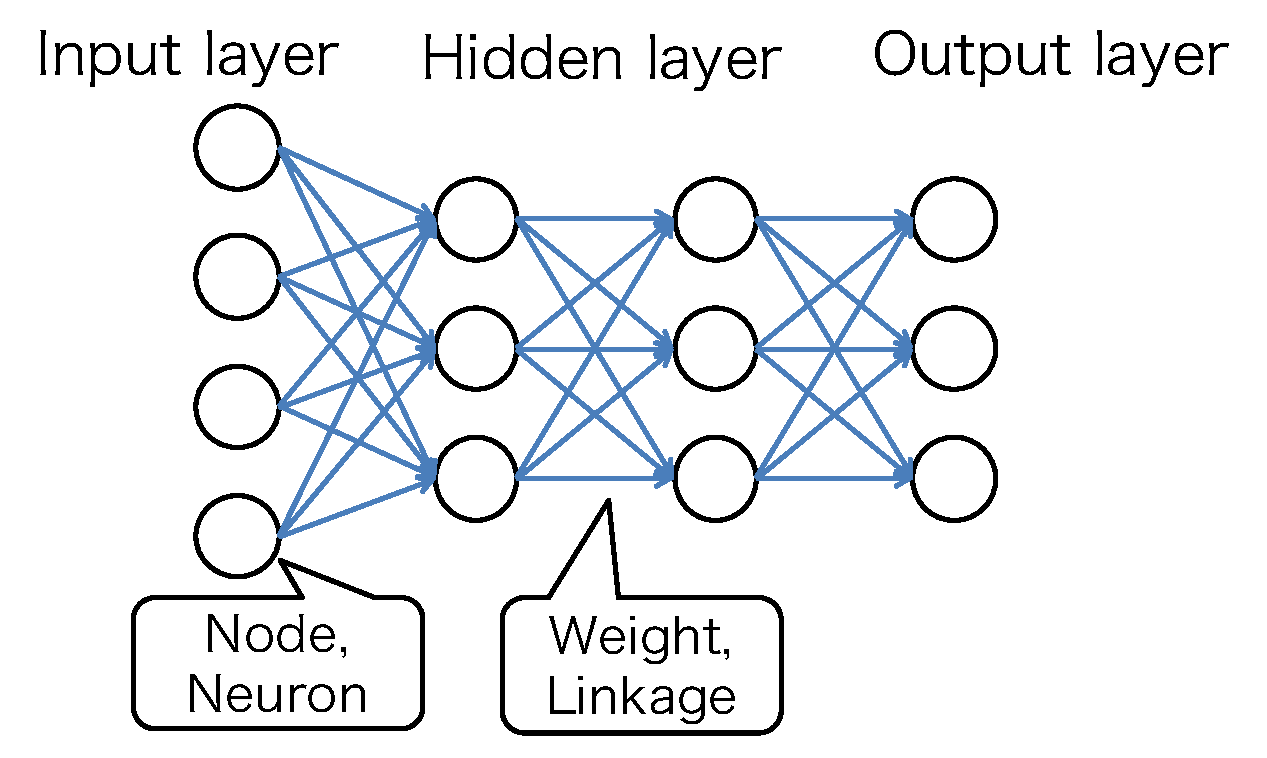
\includegraphics[width=1.2\linewidth]{fig/MLP}
		\subcaption{Muti-layer perceptron}
		\label{fig:mlp}
	\end{minipage}
	\begin{minipage}[b]{0.4\columnwidth}
		\centering
		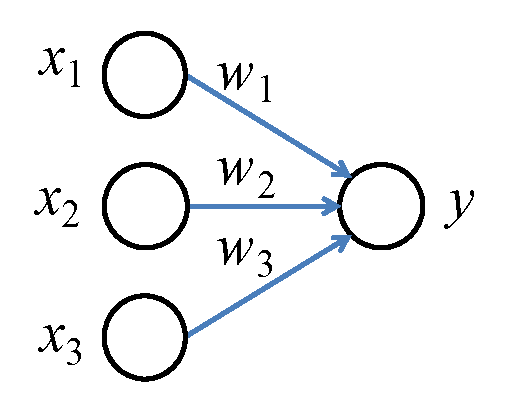
\includegraphics[width=0.7\linewidth]{fig/simple_perceptron}
		\subcaption{Simple perceptron}
		\label{fig:perceptron}
	\end{minipage}
	\caption{Architecture of Muti-layer perceptron}
\end{figure}

\fig {mlp}における丸や矢印はそれぞれノード(またはニューロン)と重み(または結合)と呼び,ともに数値である.例えば画像を分類しようと思えば,各ピクセルの画素数を各ノードに入力する.例えば$28 \times 28$pixelのグレースケール画像であれば,784個のノードが必要となる.入力データ$\bm {x}$が入力層に入ってくると,その値に重み$\bm {w}$をかけ,活性化関数$H$と呼ばれる関数に通し,結果$\bm{y}$を出力する.ここで,入力$\bm{x}$,重み$\bm{w}$,出力$\bm{y}$を太字で表したが,これらは全てテンソルであり,1つの層にあるノード$x_1, x_2, \cdots x_n$を一括して$\bm {x}$として表記している.

ここで,中間層の1つのノードについて考える.\fig {perceptron}にMLPを構成する1ユニットである単純パーセプトロンを示した.この模式図を数式で表すと次のようになる.
\begin{align}
	y & = H(\bm{w}\bm{x} + \bm{b}) \\
	& = H\left( \sum_{i=1}^3 w_i x_i + b_i \right) 
\end{align}
ここで$\bm{b}$はバイアスと呼ばれ,発火のしやすさを表している.中間層における活性化関数は,\eq {ReLU}に示す正規化線形関数(rectified linear unit: ReLU)と呼ばれる関数)がよく用いられる.
\begin{align}\label{eq:ReLU}
	H(x) = \max \left\lbrace 0, x \right\rbrace = \begin{cases}
	x & (x > 0) \\
	0 & (x \leq 0)
	\end{cases}
\end{align}
この演算を繰り返し出力層に書き出す.ここで,各層の重みの値によって出力結果は異なってくる.

出力層では,ノードの個数は区別したいクラス数分用意する.
各ノードの出力値が各クラスに属している確率を表すように,活性化関数にはソフトマックス関数を用いる(ただし二値分類の場合はシグモイド関数を用いる).ソフトマックス関数は\eq {softmax}で表される.
\begin{align}\label{eq:softmax}
	y_i = \dfrac{\exp(x_i)}{\displaystyle \sum_{k=1}^n \exp(x_k)}
\end{align}
ここで$y_i$は,出力層が全部で$n$個あるとして,$i$番目の出力であることを示す.\eq {softmax}からわかるように,入力の総和に対して1つのノードがどれくらいの値を持つかという割合で表されている.これにより各ノードの出力は確率として解釈できるため,値の一番大きいノードのインデックスを予測ラベルとして見ることができる.


\subsection{畳み込みニューラルネットワーク}
従来の画像認識では,画像から特徴を抽出しそれを識別器にかける手法が主流であった.古典的手法では画像から特徴を抽出するいわゆる特徴量設計が必要で,ここをいかにうまく設計するかがポイントであった.特徴抽出の方法として,HOG\cite{HOG}やSIFT\cite{SIFT},SURF\cite{SURF}などがあり,これらによって抽出した特徴ベクトルをSupport Vector Machine(SVM)\cite{SVM}によって識別することが多かった.

しかし,1998年にLeNetと呼ばれる畳み込みニューラルネットワーク(Convolutional Neural Network: CNN)が提案された\cite{LeNet}.CNNは畳み込み層とプーリング層からなっている.この畳み込みとプーリングの演算を通して,特徴量設計から識別までをend-to-endで行うことができる.
\begin{figure}[H]
	\centering
	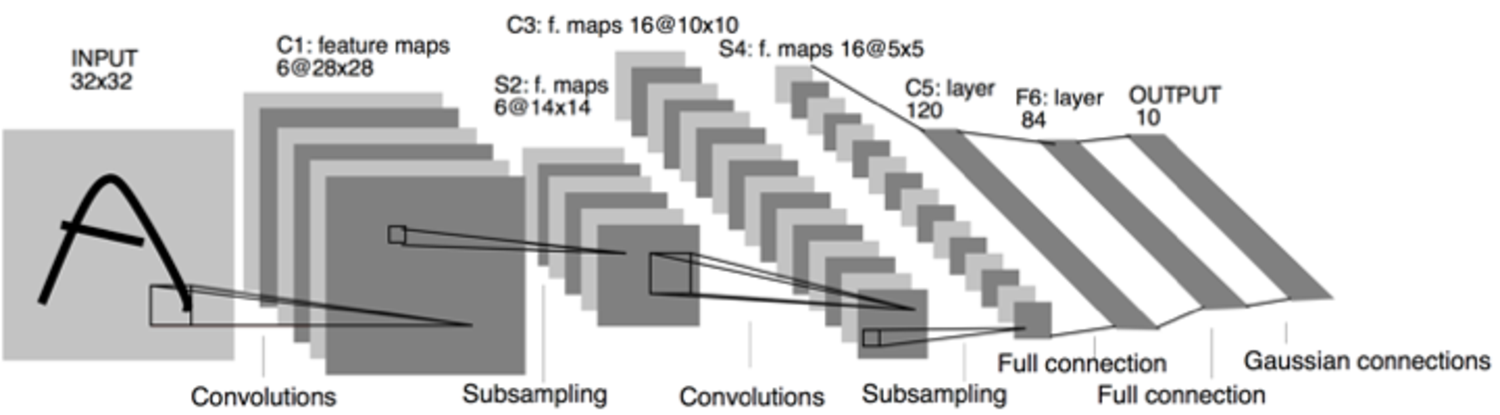
\includegraphics[width=0.7\linewidth]{fig/LeNet}
	\caption{Architecture of convolutional neural network\cite{LeNet}}
	\label{fig:LeNet}
\end{figure}


%人間が物体を認識することをコンピュータにも計算させるには,画像の特徴的な部分を切り分けて数値化させる必要がある.例えば,カラー画像の場合,RGBの3色(3チャンネル)を組み合わせた画像で認識をしている.このようなフィルターの畳み込み計算を行うと,フィルターごとに異なった画像の特徴を抽出して数値化する.これが畳み込み(convolution)である.その後,画像のサイズを小さくしてコンピュータが計算コストを減らし,微小な変化に対してロバストになる仕組みしてプーリングという方法を用いる.

畳み込み層では,入力に対してフィルター(カーネルとも呼ばれる)を用意し,\eq {conv}に示す計算を行う.
\begin{align}\label{eq:conv}
	y_{i,j} & = (\bm{K} * \bm{x})_{i,j}\\
	& = \sum_m\sum_n x_{i+m, j+n} K_{m,n}
\end{align}
ここで,$\bm{K}$はフィルター,$\bm{x}$は入力,$y$は出力である.CNNではこの演算の後に活性化関数に通す.これを図で表すと\fig {conv}のようになる.

\begin{figure}[H]
	\centering
	\begin{minipage}{0.45\columnwidth}
		\centering
		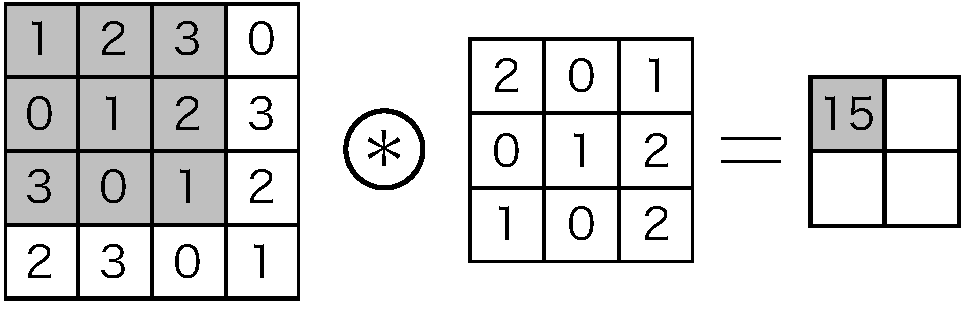
\includegraphics[width=\linewidth]{fig/conv_ex1}
		\subcaption{}
		\label{fig:conv_ex1}
	\end{minipage}
	\hspace{10truemm}
	\begin{minipage}{0.45\columnwidth}
		\centering
		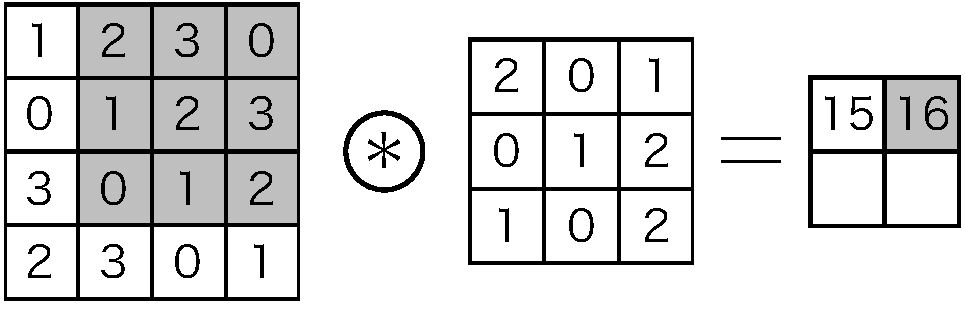
\includegraphics[width=\linewidth]{fig/conv_ex2}
		\subcaption{}
		\label{fig:conv_ex2}
	\end{minipage}
	\begin{minipage}{0.45\columnwidth}
		\centering
		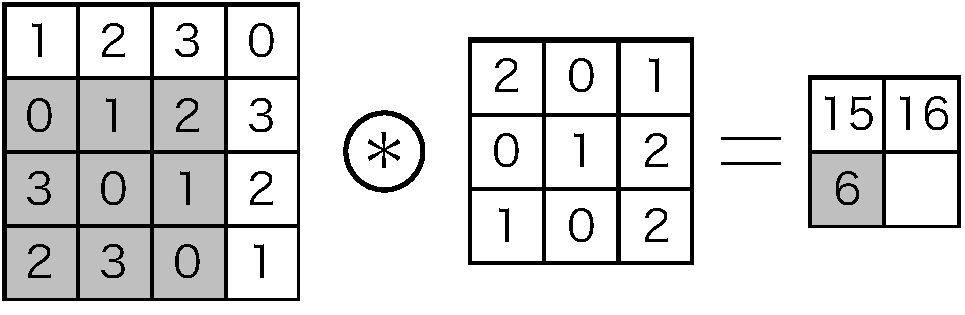
\includegraphics[width=\linewidth]{fig/conv_ex3}
		\subcaption{}
		\label{fig:conv_ex3}
	\end{minipage}
	\hspace{10truemm}
	\begin{minipage}{0.45\columnwidth}
		\centering
		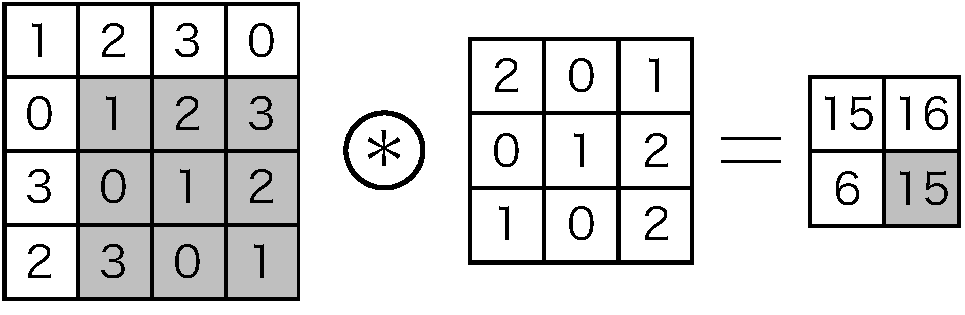
\includegraphics[width=\linewidth]{fig/conv_ex4}
		\subcaption{}
		\label{fig:conv_ex4}
	\end{minipage}
	\caption{Operation process of convolution}
	\label{fig:conv}
\end{figure}

\fig {conv}では,フィルターのサイズは$3\times 3$であるが,大きさは任意である($3\times 3$や$5\times 5$, $7\times 7$がよく用いられる).また,フィルターは1マスずつ横にずらして計算を行っている.ずらし方をストライドといい,今回はストライド1である.CNNでは多くの場合,ストライドは1である.
このようなフィルターの畳み込み計算を行うと,フィルターごとに異なった画像の特徴を抽出して数値化することができる.

次にプーリングを行う.ここでは,画像認識で多く用いられる最大値プーリングについて述べる.\fig {pooling}に示すように,$2\times 2$のプールサイズを用意した時,その範囲内にある最大値を取る演算である.ストライドはプールサイズと合わせ,プーリングを行った領域と被らないようにすることが一般的である.\fig {pooling}ではストライド2である.

\begin{figure}[H]
	\centering
	\begin{minipage}[b]{0.4\columnwidth}
		\centering
		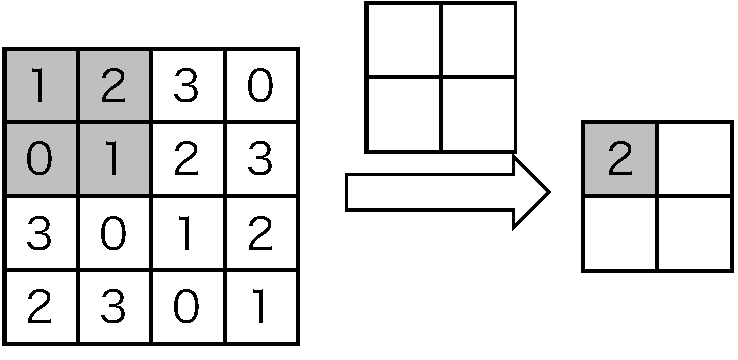
\includegraphics[width=\linewidth]{fig/pooling_ex1}
		\subcaption{}
		\label{fig:pooling_ex1}
	\end{minipage}
	\hspace{10truemm}
	\begin{minipage}[b]{0.4\columnwidth}
		\centering
		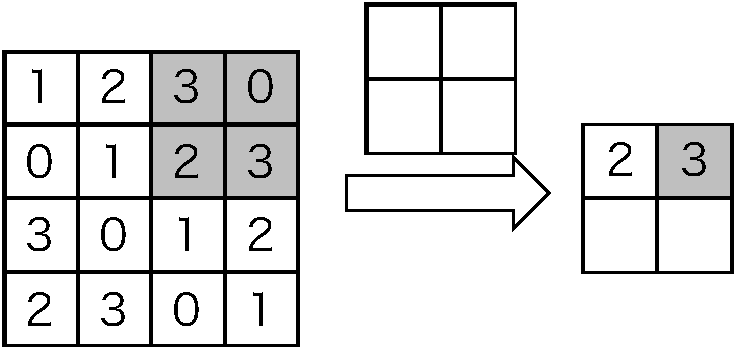
\includegraphics[width=\linewidth]{fig/pooling_ex2}
		\subcaption{}
		\label{fig:pooling_ex2}
	\end{minipage}
	\begin{minipage}[b]{0.4\columnwidth}
		\centering
		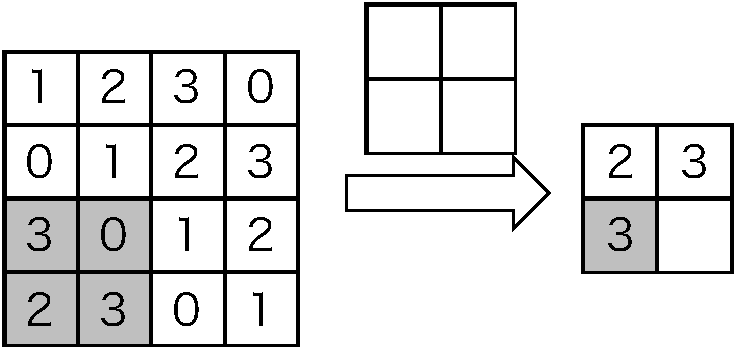
\includegraphics[width=\linewidth]{fig/pooling_ex3}
		\subcaption{}
		\label{fig:pooling_ex3}
	\end{minipage}
	\hspace{10truemm}
	\begin{minipage}[b]{0.4\columnwidth}
		\centering
		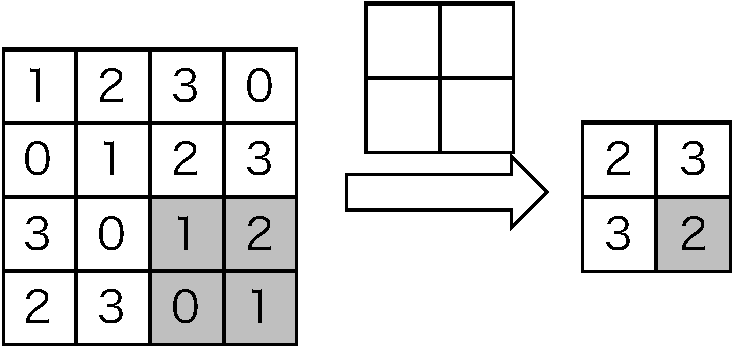
\includegraphics[width=\linewidth]{fig/pooling_ex4}
		\subcaption{}
		\label{fig:pooling_ex4}
	\end{minipage}
	\caption{Operation process of max pooling}
	\label{fig:maxpooling}
\end{figure}

プーリング層では画像のサイズを小さくして(コンピュータの)計算コストを減らし,微小な変化に対してロバストになる.

この畳み込みとプーリングを繰り返して,入力からフィルターの数だけ特徴を抽出し,この抽出した特徴マップをFC層へ繋げて識別を行う手法がCNNである.


\subsection{再帰的ニューラルネットワーク}
再帰的ニューラルネットワーク(Recurrent Neural Network: RNN)は時系列解析や自然言語処理に利用されるニューラルネットワークである.\fig {simpleRNN}に示すように,内部にループを持つことで過去の情報を保持しておくことができる.

\begin{figure}[H]
	\centering
	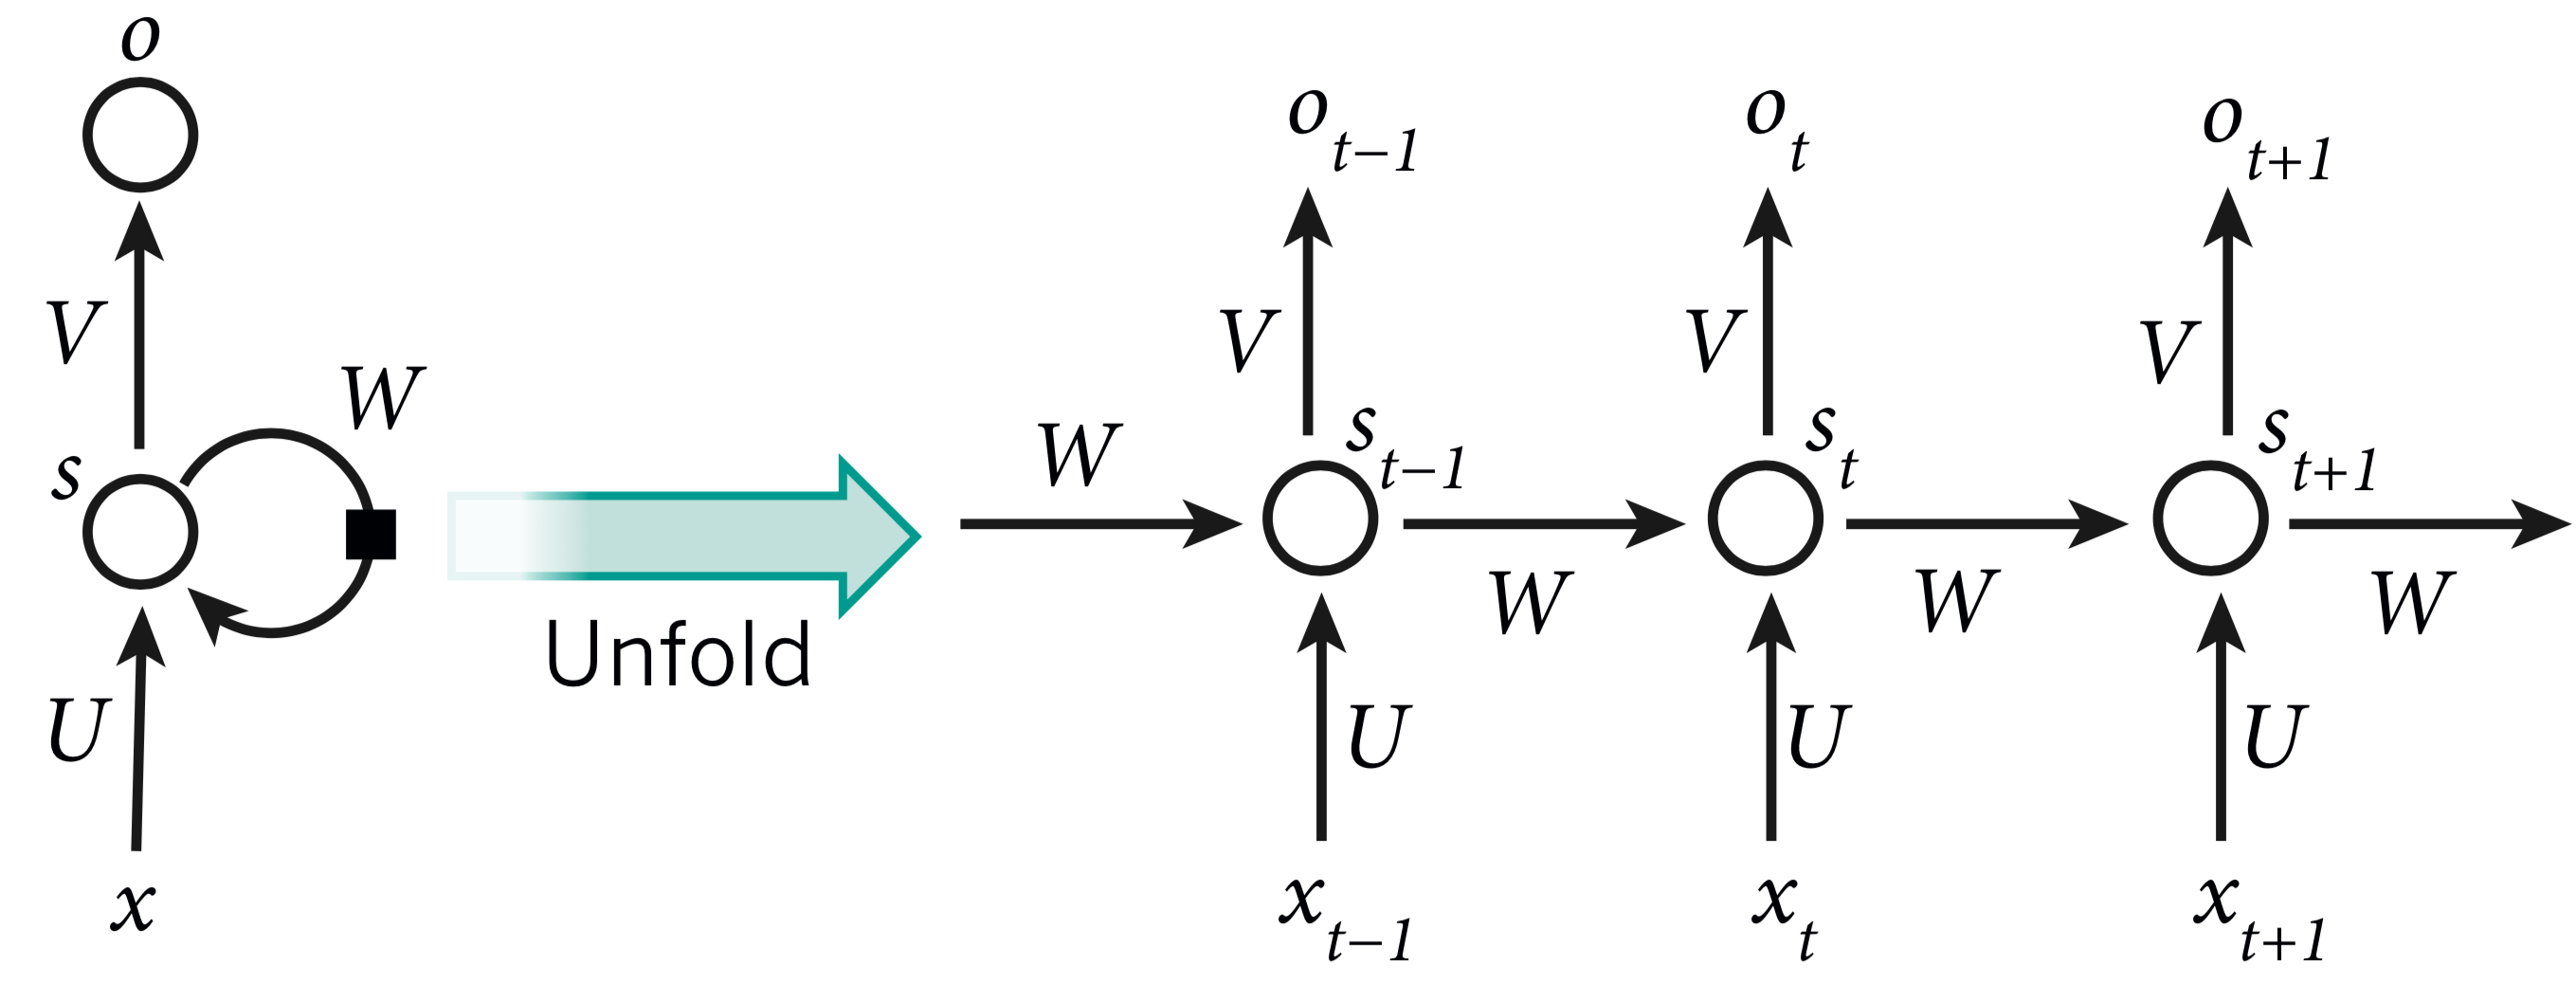
\includegraphics[width=0.7\linewidth]{fig/simpleRNN}
	\caption{Architecture of RNN\cite{simpleRNN}}
	\label{fig:simpleRNN}
\end{figure}


時系列の入力$\bm{x} = (x_1, \cdots , x_T)$があった時に,出力$\bm{y} = (y_1, \cdots , y_T)$と隠れ層のベクトル$\bm{h} = (h1, \cdots ,h_T)$をそれぞれ以下の式で計算する.

\begin{align}\label{eq:RNN}
	h_t & = H(W_{ih} x_t + W_{hh} h_{t-1} + b_h) \\ 
	y_t & = W_{ho} h_t + b_o
\end{align}

ここで,$\bm{W}$は重み行列($W_{ih}$は入力と隠れ層間の重み行列)であり,$\bm{b}$はバイアス項,$H$は活性化関数である.

\subsection*{LSTM}
RNNは,過去の情報をどこまで遡って関連性を見つけるか判断することができない.そのため,時系列データが長くなるほどその長期の依存性を学習するには人が慎重にパラメータを設計する必要があり,長期的なデータは学習が難しい問題があった.この問題を解決するためにLong-short term memory(LSTM)が提案された.\fig {LSTM}に示すように,LSTMもRNNの一種であるため繰り返し構造を持ち,3つのゲートを持つ層からなっている.

\begin{figure}[h]
	\centering
	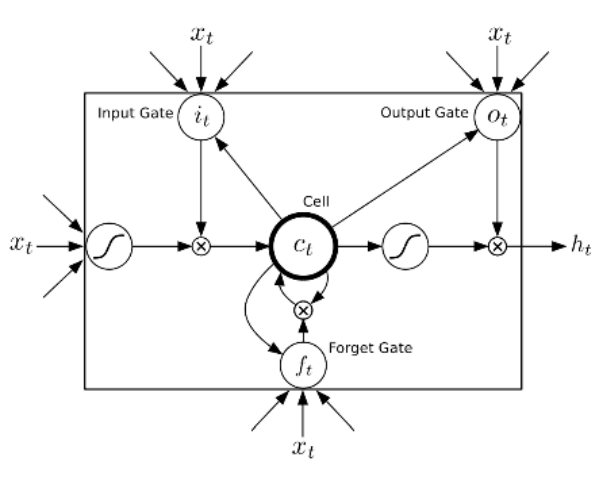
\includegraphics[width=0.7\linewidth]{fig/lstm.png}
	\caption{Architecture of LSTM}
	\label{fig:LSTM}
\end{figure}

\begin{align}\label{eq:LSTM}
	f_t & = \sigma(W_{xf} x_t + W_{hf} h_{t-1} + W_{cf} c_{t-1} + b_f ) \\
	i_t & = \sigma(W_{xi} x_t + W_{hi} h_{t-1} + W_{ci} c_{t-1} + b_i) \\
	c_t & = f_t c_{t-1} + i_t \tanh(W_{xc} x_t + W_{hc} h_{t-1} + b_c) \\
	o_t & = \sigma(W_{xo} x_t + W_{ho} h_{t-1} + W_{co} c_t + b_o) \\
	h_t & = o_t \tanh(c_t) 
\end{align}

ここで,活性化関数にはシグモイド関数および$\tanh$を用いる.シグモイド関数は次の式で定義される.
\begin{equation}\label{eq:sigmoid}
	\sigma (x) = \dfrac{1}{1 + e^{-x}}
\end{equation}

$f_t$で示される層は忘却ゲート層と呼ばれ,過去の情報で捨てるべき情報を判断する.これはシグモイド層によって行われ,0と1の間の値を出力し,0は完全に忘れる.1は完全に維持するという意味である.
$i_t$や$c_t$で示される層は,入力ゲート層と呼ばれ,$i_t$で新たに入力された情報から,どの情報を更新するかを判断し,$c_t$で古い情報を落とし新しい情報を加え値を更新する.
最後が$o_t$や$h_t$で示される層で,出力ゲート層と呼ばれる.まず何を出力するべきかを$o_t$のゲートで判断して,$c_t$に$\tanh$を適用して掛けることで出力が計算される.

\subsection*{GRU}


\section{推論と学習}
ニューラルネットワークでは推論フェーズと学習フェーズに分かれている.\ref{sec:NeuralNetwork}節は全て推論フェーズの話であり,順伝播ニューラルネットと呼ばれる.

学習フェーズでは,逆伝播ニューラルネットを用いる.逆伝播とは誤差逆伝播法(Backpropergation)\cite{Backprop}から由来している.真値からの誤差を表す損失関数(loss function)を用いて,パラメータの微分値を更新に用いる.損失関数はコスト関数,目的関数とも呼ばれる.この微分値を効率よく計算するアルゴリズムが誤差逆伝播法である.

損失関数は解く問題の目的に合わせて選ぶ必要がある.回帰問題では平均二乗和誤差(mean squared error: MSE)が用いられる.
\begin{align}\label{eq:mse}
	L_{\mathrm{MSE}} = \dfrac{1}{2} \sum_{k} (y_k - t_k)^2
\end{align}
また,クラス分け問題では交差エントロピー誤差(cross entropy error)が用いられる.
\begin{align}\label{eq:crossentropy}
	L_{\mathrm{cross}} = - \sum_k t_k \ln {y_k}
\end{align}
ここで,$y$は予測ラベルで,$t$は教師ラベルである.

\subsection{最適化手法}
損失関数を用いてパラメータを更新するが,更新手法にはいくつか方法があるため,ここでは本研究で使用した最適化手法について述べる.

\subsection*{SGD}
SGDは日本語で確率的勾配降下法(Stochastic gradient descent)と呼ばれる手法で,最も単純な最適化手法である.画像認識の分野では多く使われている.

SGDでは以下の式\eq {SGD}でパラメータを更新する.
\begin{align}\label{eq:SGD}
	\bm{W} \leftarrow \bm{W} - \eta \pdif{L}{\bm{W}} 
\end{align}
ここで,$\bm{W}$は更新する重みパラメータ,$\pdif{L}{\bm{W}}$は$\bm{W}$に関する損失関数の勾配である.また$\eta$は学習率と呼ばれ,実際には0.01や0.001といった値を前もって決めて使用する.SGDはパラメータの勾配を利用して,勾配方向にパラメータを更新するステップを繰り返して,徐々に最適なパラメータへと近づける手法である.

\subsection*{Adam}
Adam\cite{Adam}はadaptive moment estimationの略で,勾配の値の1乗和と2乗和の両方をパラメータ更新に用いる手法である.以下の式\eq{adam}でパラメータを更新する.

\begin{align}\label{eq:adam}
	\bm{m} & \leftarrow \beta_1 \bm{m} + (1 - \beta_1) \pdif{L}{\bm{W}} \\
	\bm{v} & \leftarrow \beta_2 \bm{v} + (1 - \beta_2) \left( \pdif{L}{\bm{W}} \right) ^2 \\
	\bm{W} & \leftarrow \bm{W} - \eta \dfrac{\hat{\bm{m}}}{\sqrt{\hat{\bm{v}}} + \epsilon} 
\end{align}

$m_t$と$v_t$はそれぞれ、勾配の一次モーメント(平均値)と二次モーメント(分散した平方偏差)の概算値である.$\eta$,$\beta_1$,$\beta_2$はそれぞれ学習パラメータである.
また,$\hat{m}_t$,$\hat{v}_t$はそれぞれ移動指数平均を用いた際に生じるバイアス(大きさを変えてしまっていることなど)を打ち消すために正則化しており,\eq {adamhat}で表される.

\begin{align}\label{eq:adamhat}
	\hat{\bm{m}} & = \dfrac{\bm{m}}{1 - \beta_1} \\
	\hat{\bm{v}} & = \dfrac{\bm{v}}{1 - \beta_2}
\end{align}

学習パラメータはそれぞれ$\eta = 0.001$,$\beta_1 = 0.9$,$\beta_2 = 0.999$,$\epsilon = 10^{-8}$が最適だと言われている\cite{Adam}.

\subsection{学習のテクニック}
ディープラーニングでは過学習(overfitting)と呼ばれる問題が多く起こる.過学習とは,訓練データに対してのみ適応し過ぎてしまい,訓練データに含まれないテストデータには精度が出ない状態を指す.過学習は,大量にパラメータを持つ表現力の高いモデルであることや,訓練データが少ないことなどが原因で起こる.ここでは過学習を抑制するテクニックを述べる.
\subsection*{Dropout}
Dropout\cite{Dropout}は,ネットワークのノードをランダムに消去しながら学習する手法である.訓練時に隠れ層のノードを毎回ランダムに選択し,そのノードの出力を0にする.そしてテスト時には全てのノードを活性化させ,信号を伝達させる.

Dropoutは,学習時にノードをランダムに消去することで,毎回異なるモデルを学習していると解釈でき,アンサンブル学習と同じ効果を擬似的に1つのネットワークで実現していると考えられる.アンサンブル学習とは,弱識別器を複数合わせて1つの強力な識別器とする手法で,現在でも有効な手法として用いられている.

\subsection*{Batch Normalization}
Batch Normalization\cite{BatchNorm}は,ネットワークにおける各層での活性化後の出力(アクティベーション)の分布を,適度な広がりを持つように調整する手法である.Batch Normalizationでは学習を行う際のミニバッチを単位として,ミニバッチごとに正規化を行う(\eq {BatchNorm}).
\begin{align}\label{eq:BatchNorm}
	\mu_B & = \dfrac{1}{m}\sum_{i=1}^m x_i \\
	\sigma_B^2 & = \dfrac{1}{m}\sum_{i=1}^m (x_i - \mu_B) \\
	\hat{x_i} & \leftarrow \dfrac{x_i - \mu_B}{\sqrt{\sigma_B^2 + \epsilon}}
\end{align}
ミニバッチとして$B = \{x_1, x_2, \cdots, x_m\}$という$m$個の入力データの集合に対して,平均$\mu_B$,分散$\sigma_B^2$を求め,入力データを平均0分散1となるように正規化を行う.$\epsilon$は0で除算されることを防ぐもので,極小の値を用いる.

Batch Normalizationを用いると,学習を速く進行させることができる,初期値にそれほど依存しない,過学習を抑制できるといった効果が期待できる.

\subsection*{Data Augumentation}
Data Augumentation(データ拡張)は,訓練データを人工的に水増しする手法である.例えば,入力画像に対して回転や縦横の移動,上下反転,鏡面反転などの操作をして訓練データを擬似的に増やす.これは,ニューラルネットは大きな位置ずれや対象物が回転した状態にあると別のものとして認識してしまうことを逆手にとった手法である.訓練データが少ないときに大きな効果を発揮する.


\section{画像認識におけるディープラーニング}
%教師あり学習であることもここで触れておきたい
Deep LearningとはDeep Neural Network(DNN)を指すことが多い.この"Deep"とは,ニューラルネットワークの層が深いことに由来している.

\fig {ImageNet}に画像認識タスクの精度の近年の推移を示す.これはImageNet Large Scale Visual Recognition Challenge (ILSVRC)と呼ばれる世界的な画像認識のコンペティションである(2010年から始まった).カテゴリ数は1000クラスで,画像枚数は120万枚の訓練データと15万枚のテストデータが用意されている.
\begin{figure}[H]
	\centering
	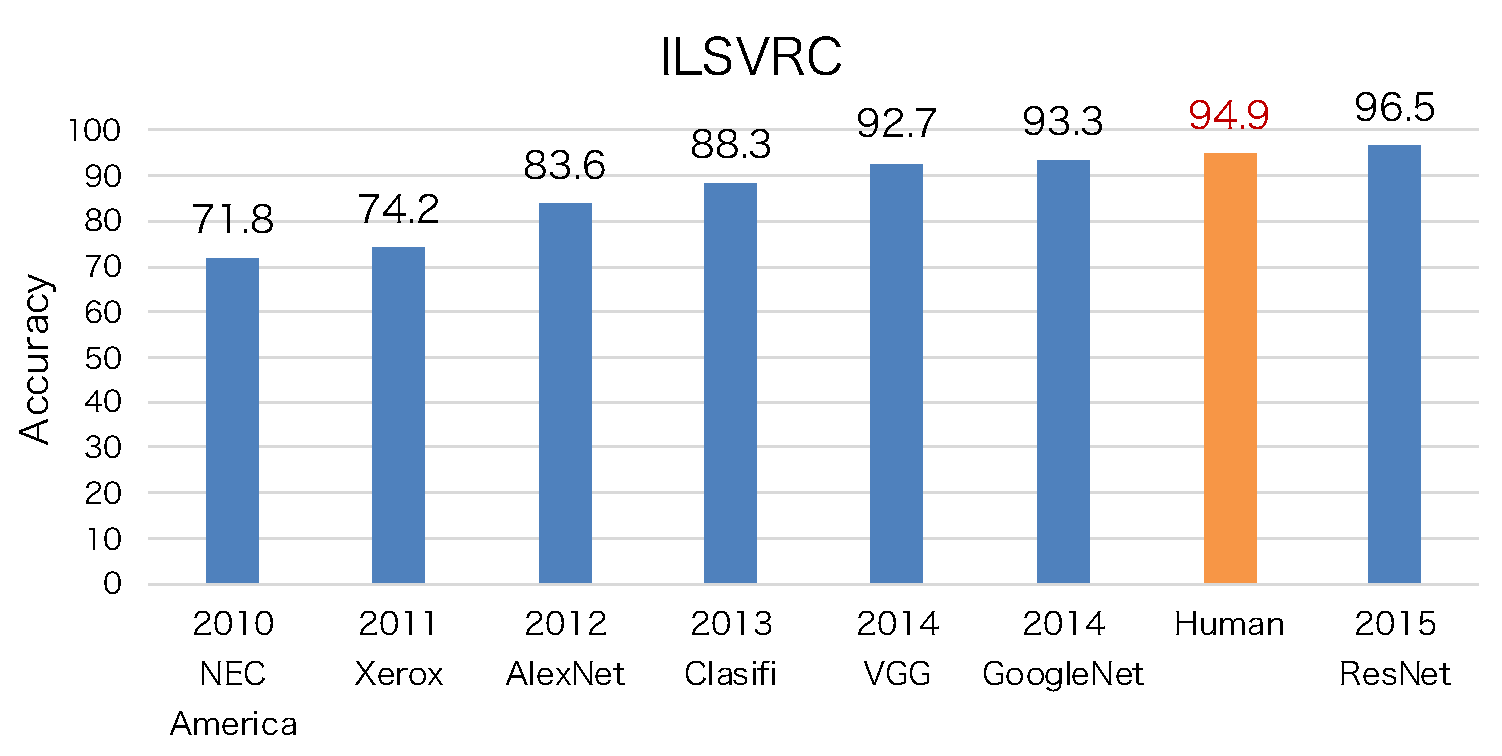
\includegraphics[width=0.7\linewidth]{fig/ILSVRC}
	\caption{Transition of accuracy of image recognition on ILSVRC}
	\label{fig:ImageNet}
\end{figure}
2011年と2012年は約10\%もの大差でAlexNet\cite{AlexNet}が優勝している.これがディープラーニングの始まりである.AlexNetは5つの畳み込み層と3つの全結合層を持っている.2014年にはVGGNet\cite{VGGNet}やGoogLeNet\cite{GoogLeNet}が9割の精度を超えた.VGGNetはAlexNet(8層)よりさらに深い構造(19層)であり,GoogLeNetは22層もある.そして2015年にはResNet\cite{ResNet}が人間の精度をも超える認識精度を達成した.ResNetはGoogLeNetよりもさらに深く152層もある.CNNを複数回かけて検出を行う場合,CNNの浅い側では空間分解能はあるが抽象的な情報が少ない.深い側では意味論的な情報は取得できる(ポーズ,変形など)が空間分解能が小さいため幾何学的な情報が失われる.

アーキテクチャの進化の方向は大きく3つある.1つ目は層を深くすることである.
2つ目はFC層の使用を避ける,またはInceptionモジュールの使用することである.これにより学習するパラメータ数を削減することができる.3つ目はResNetなどのショートカット接続の利用や,事前学習・転移学習を行うことである.これによって学習効率を向上させ,最終的にモデルの精度向上へと繋がる.ここで,事前学習のデータセットと適用データとの間には類似性があると良い.

画像処理におけるディープラーニングでは大きく3つのタスクがあり,それぞれ,クラス分類,物体検出,セグメンテーションである.以下に詳細を述べる.

\subsection*{クラス分類}
与えられた画像をカテゴリごとに分ける手法である.

\subsection*{物体検出}
物体検出とはBounding Boxで物体の位置とその物体の種類を特定する方法である.歴史的には幾何的情報,手動特徴量,そしてそのカスケードを利用していた.その後,HOGやSIFTなど局所特徴量を抽出する方法を設計するようになったが,これは深い専門知識を必要とした.また広い範囲でオブジェクトを正確に検出する方法は,メモリ容量と処理時間に課題がある.現在はDeep Neural Networkになりデータのみから抽象的な特徴量を複数得ることができる.\fig {YOLO}に物体検出で有名はアルゴリズムであるSSDとYOLOのアーキテクチャを示す.クラス分けの場合は数1000のカテゴリを学習してTop Error Rateが2\%以下と人間よりも認識精度が高いが,物体検出においては,現状ではカテゴリが数100程度くらいまででも認識精度が人間よりも低くなってしまう.また物体検出は精度を上げるために処理に時間がかかることが多いため,リアルタイムに物体検出を行う時は,速度と精度のトレードオフが生じてしまう.

\begin{figure}[H]
	\centering
	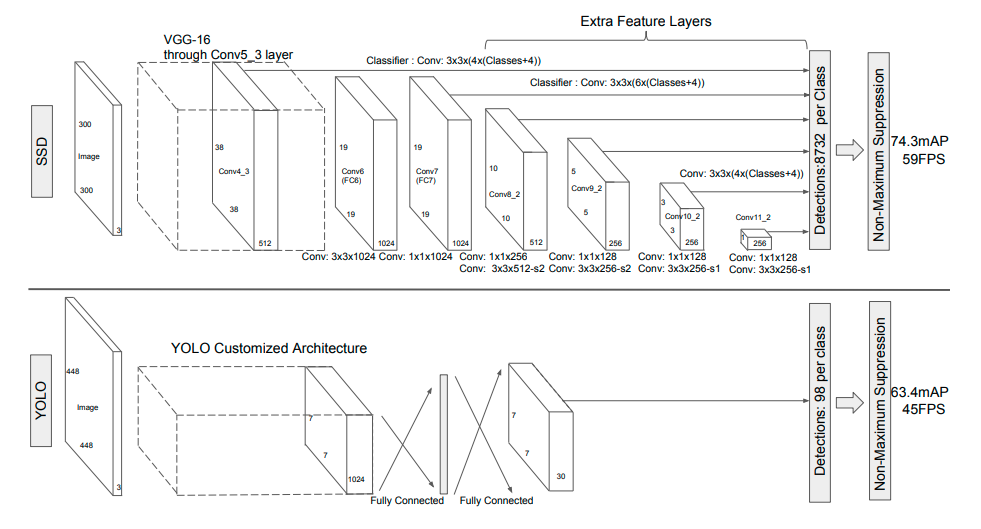
\includegraphics[width=0.7\linewidth]{fig/yolo_ssd.png}
	\caption{Network Architecture of SSD and YOLO}
	\label{fig:YOLO}
\end{figure}

\subsection*{セグメンテーション}
セマンティックセグメンテーションとは,画像を画素レベルで認識することである.画像内の各画素をオブジェクトクラスに割り当てる手法である.セマンティックセグメンテーションの手法についてディープラーニング以前では,Texton Forestsや,Random Forestsに基づいた分類を行っていたが,物体検出と同様にCNNが登場してからは,高精度なセグメンテーションが実現するようになった.CNNを使ったセグメンテーションの手法で一般的に使われるようになったものがUnetである(\fig {Unet}).このUnetは文字通りUの形をしたネットワークであることが特徴で,2つのアーキテクチャーからできている.1つ目がエンコーダーのアーキテクチャーでCNNとプーリングで特徴を抽出しながら次元を削減していき,2つ目のデコーダーのアーキテクチャーで画像をセグメンテーションの結果になるように復元する.ここで問題になることが,プーリングをすることで位置情報を消してしまっているので,この位置情報を利用して画像を復元するためには,エンコーダーとデコーダーで画像サイズが同じところ同士をショートカットで接続することがUnet構造の優れている点である.

\begin{figure}[H]
	\centering
	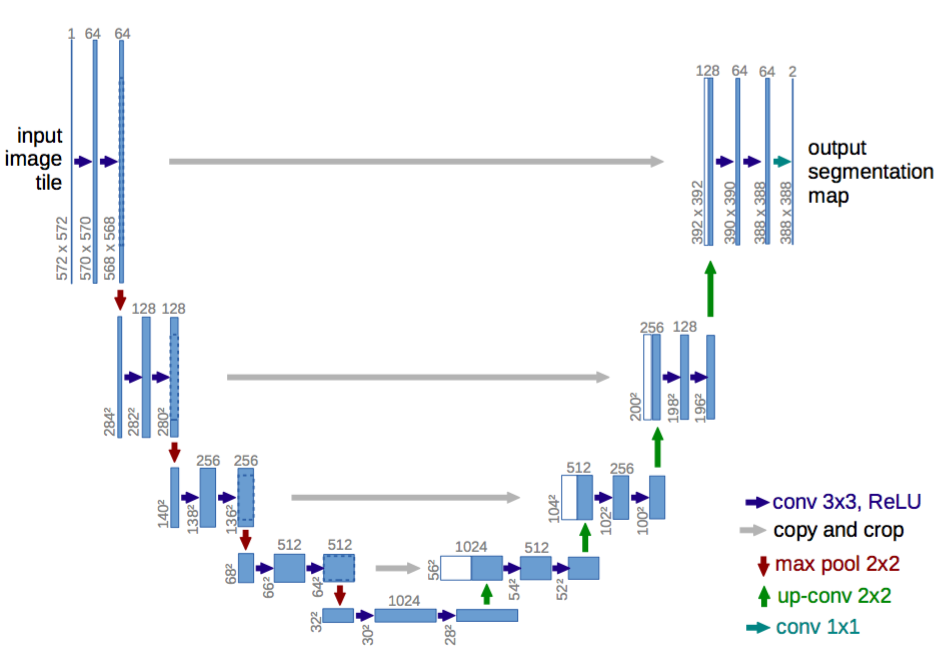
\includegraphics[width=0.7\linewidth]{fig/unet.png}
	\caption{Artchitecture of Unet}
	\label{fig:Unet}
\end{figure}

\section{深層学習による3次元画像解析}
ディープラーニングを医療画像に応用するコンペティションが世界で行われているが,その半数が3D医療画像の解析になっているほど需要が高まっている.その理由は,現在解決しなくてはならない課題があるからである.まずは2次元画像と違って,処理するべきデータが大きいということである.そのため学習するパラメータをなるべく少なくする工夫がされている.また3次元画像には,動画または,ボリューム画像があるが,2次元画像とその深さ方向(動画であれば,時間方向)には異方性があることから,機械学習の方法に工夫が必要になる.今まで考案されている手法として,2DCNNを拡張した3DCNN,またCNNと時系列解析でよく用いられるLSTMを組み合わせた手法と,LSTM内部にCNNを組み込んだ手法,それらをすべて組み合わせた手法が考案されいる.LSTMの研究も盛んに行われているため,その改良モデルが数多く存在する.特に,LSTMの学習効率を上げたGRU(Gated Linear Unit)や,順方向だけでなく逆方向の時系列も計算に入れるBiLSTMが時系列解析の精度向上になっている報告がある.


\subsection{3DCNNとStacked Convolution}
2次元画像が深さ方向に連続している3次元画像の特徴を抽出するために,2次元のCNNを拡張して,3次元のカーネルを使って畳み込みを行う,3DCNNを利用した手法がある.

\begin{figure}[H]
	\centering
	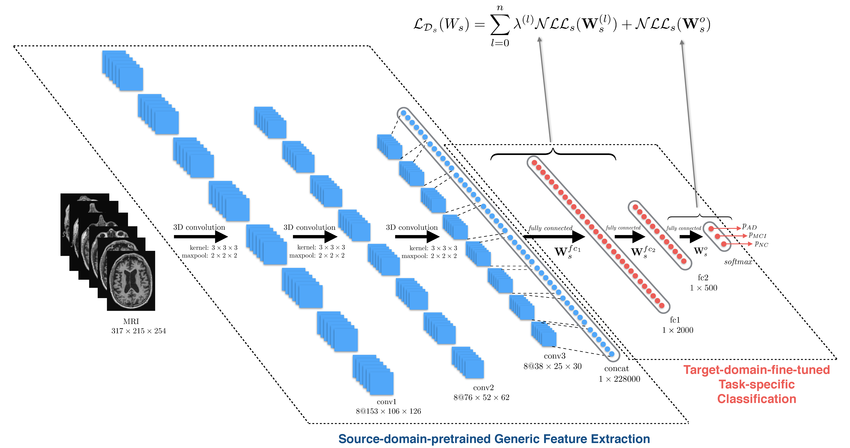
\includegraphics[width=0.7\linewidth]{fig/3d_cnn.png}
	\caption{Artchitecture of 3DCNN}
	\label{fig:3DCNN}
\end{figure}


\begin{figure}[H]
	\centering
	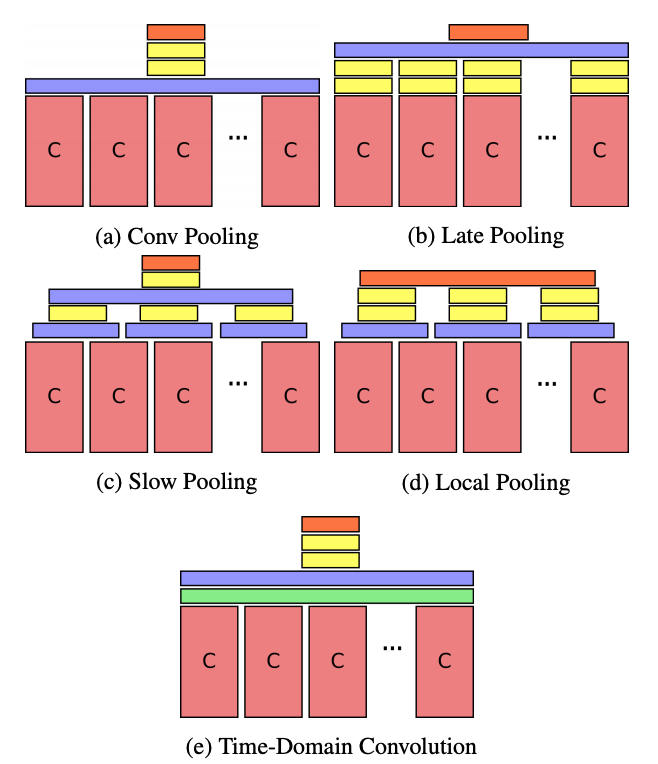
\includegraphics[width=0.7\linewidth]{fig/stacked_conv.png}
	\caption{Architecture of stacked convolution}
	\label{fig:stacked_conv}
\end{figure}

\subsection{LSTMと2DCNNの組み合わせ}
時系列解析に使われるLSTMを用いて3次元の画像を解析することができる.これはよく動画の解析で行われることがある.つまりフレームごとの画像の特徴を2次元のCNNで計算してから時系列情報をLSTMで解析することで,画像の時系列解析を行うことができる.これを3次元の医療画像でCTやMRIで適用する研究も行われている.3DCNNのデメリットであったパラメータの増大を2DCNNとLSTMの組み合わせで解決することができる.

\section{教師なし学習}
機械学習の手法には,上記で説明したように,ラベルの貼られているデータセットを用いて学習することを教師あり学習と呼び,その反対で,データセットはあっても,そのデータセットの特性を示したラベルが与えられていない場合のデータセットを用いて学習することを教師なし学習と呼ぶ.

\subsection{Autoencoder}
教師なし学習で画像の特徴を抽出する方法としてオートエンコーダがある.画像の場合におけるオートエンコーダの手法とは,ある画像から情報を圧縮する「エンコーダ」と言われる部分と,その圧縮した情報から画像を復元する「デコーダ」の二つからなる.入力とデコーダから復元された画像が同じ画像になるようにニューラルネットワークで学習させる.この学習の結果,潜在変数は似てる画像どうしで近い値になるように変化し,この分布を見れば画像の分類を教師ラベルがなくても,学習を行うことができる.

\subsection{Variational Autoencoder}
本研究では,このオートエンコーダの派生である.Variational Autoencoder(VAE)を利用した.これはオートエンコーダの「エンコーダ」と「デコーダ」は同じネットワーク構造であるが,データセットの潜在変数の分布が,正規分布になるような制約を加えて学習を行う手法である.こうすることでAutoencoderの潜在変数では分布の距離に意味ないが,VAEでは正規分布に埋め込まれるため,画像の類似度を分布が表現することができるところが特徴である.

\subsection{敵対的生成ネットワーク}
敵対的生成ネットワーク(Generative Advarsarial Network: GAN)は2014年に提案された手法である.\fig {GAN}のようにGANではGeneratorとDiscriminatorの2つのネットワークがある.Generatorは訓練データと同じような画像を生成するネットワークでDiscriminatorは,入力されたデータが訓練データから来たものかGeneratorで生成されたものかを識別するように学習する.
VAEよりもGANの方が細部まで鮮明に画像を生成することができる.しかしGANは計算時間がかかるという問題や,DiscriminatorかGeneratorのどちらかか強くなってしまうなど,学習が安定しない問題があるため,これについての多くの研究報告がされている.

\begin{figure}[H]
	\centering
	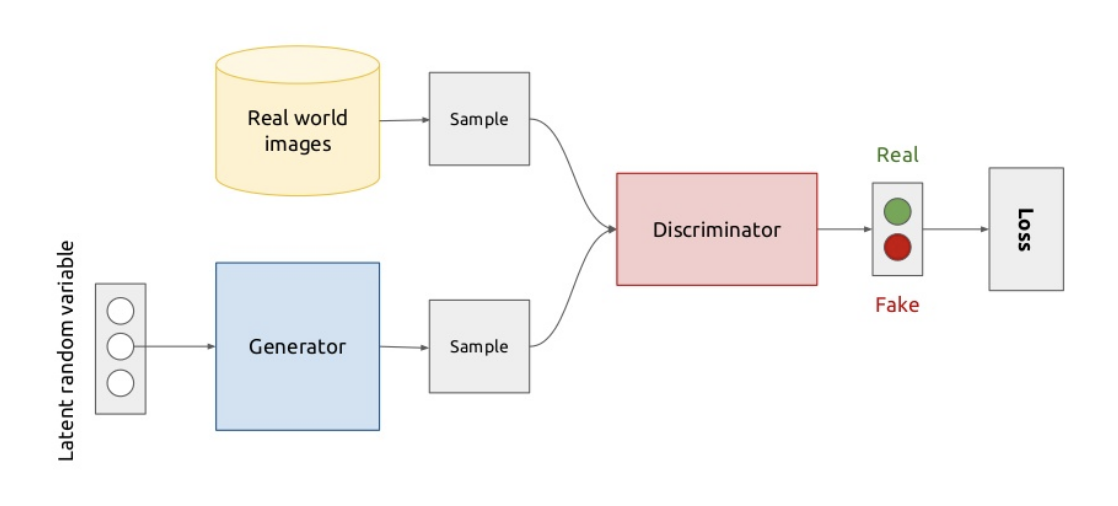
\includegraphics[width=0.7\linewidth]{fig/generative_adversarial_nets.png}
	\caption{Diagram of GAN}
	\label{fig:GAN}
\end{figure}

\section{半教師あり学習}
弱教師あり学習とも呼ばれる.これは,教師あり学習と教師なし学習を組み合わせて学習する方法である.こうすることでデータに教師ラベルをつけているものが少数であっても,データの特徴を学習しながら少量のラベルで識別境界を決めることができる.
GANやVAEの考え方を発展させてネットワークを構築することが考えられる.

\chapter{3D画像の半教師あり学習による,少量ラベルの腫瘍と正常の分類}

\section{胃がんの画像データ取得方法}

\subsection{透明化と染色}
ホルマリン固定されている検体をLUCIDによる透明化してから染色する.
多光子顕微鏡で3D画像として撮影する.一つの視野で観察することができる領域は縦横が~で深さ方向が~である.ここでLUCIDによる透明化によって今までは断面のみの撮影だったものを深さ方向まで撮影することができるようになった.
検体全ての撮影をするために画像取得にはタイリングをする.

\subsection{擬似HE染色}

\subsection{教師データの作成}

\section{古典的な画像処理手法による識別精度評価}
\subsection{2次元画像}
円検出と楕円検出を行なって,
\subsection{3次元画像}

\section{教師あり学習による識別精度評価}
\subsection{2次元画像}
\subsection{3次元画像}

\section{教師なし学習による識別精度評価}
\subsection{2次元画像}
\subsection{3次元画像}

\section{半教師あり学習による識別精度評価}
\subsection{2次元画像}
\subsection{3次元画像}


%\chapter{\LaTeX{}の使い方}
本章では、\LaTeX{}の使い方を以下説明します。\textbf{\textsf{ここでの表示例は本PDFを読むだけではどのような\LaTeX{}コードに対応しているか分かりませんので、\texttt{main.tex}や\texttt{LaTeX.tex}の中身を参照してください。}}

このPDF文書中に\texttt{command}のような書体で記載されているものは、\LaTeX{}ソース中で実際に入力するコマンドやファイル名を示しています。

\section{節の使い方}
\texttt{\bs{}section}や\texttt{\bs{}subsection}を使うと「節」(section)と呼ばれる構造を作ることができます。長い章を分割して論理展開を分かりやすくする目的で使います。

文中で節を参照するときは、\texttt{section}であっても\texttt{subsection}であっても「節」と呼び、「\ref{sec_figure}~節」や「第\ref{sec_figure}~節」のように書きます(\texttt{ref}コマンドの使用は次節参照)。章を参照するときは「\ref{chap_review}~章」や「第\ref{chap_review}~章」とします。

\section{図の使い方}
\label{sec_figure} % このようにラベルをつけることで、\refコマンドで節や図の番号を参照できます。

論文中に図を入れるときは、\texttt{figure}環境を使用します。画像形式は図~\ref{fig_CTA}のようなJPEG(主に写真などに最適)やPNG(色数の少ない画像に最適)に加え、図~\ref{fig_histogram}のようにPDF(グラフなどに最適)も使うことができます。実際の使い方は、この\LaTeX{}のコードを読んでください。\textsf{\textbf{EPS形式はいまどき誰も使いません。古い\LaTeX{}の本や年寄りに騙されないでください。}}

\begin{figure} % 特に強い理由がない限り、[htbp]のような指定はしないでください。
  \centering
  % 図の横幅をちょうど良い具合に自分で調整します。
  % 図中の文字を読めないような大きさにはしないでください。
  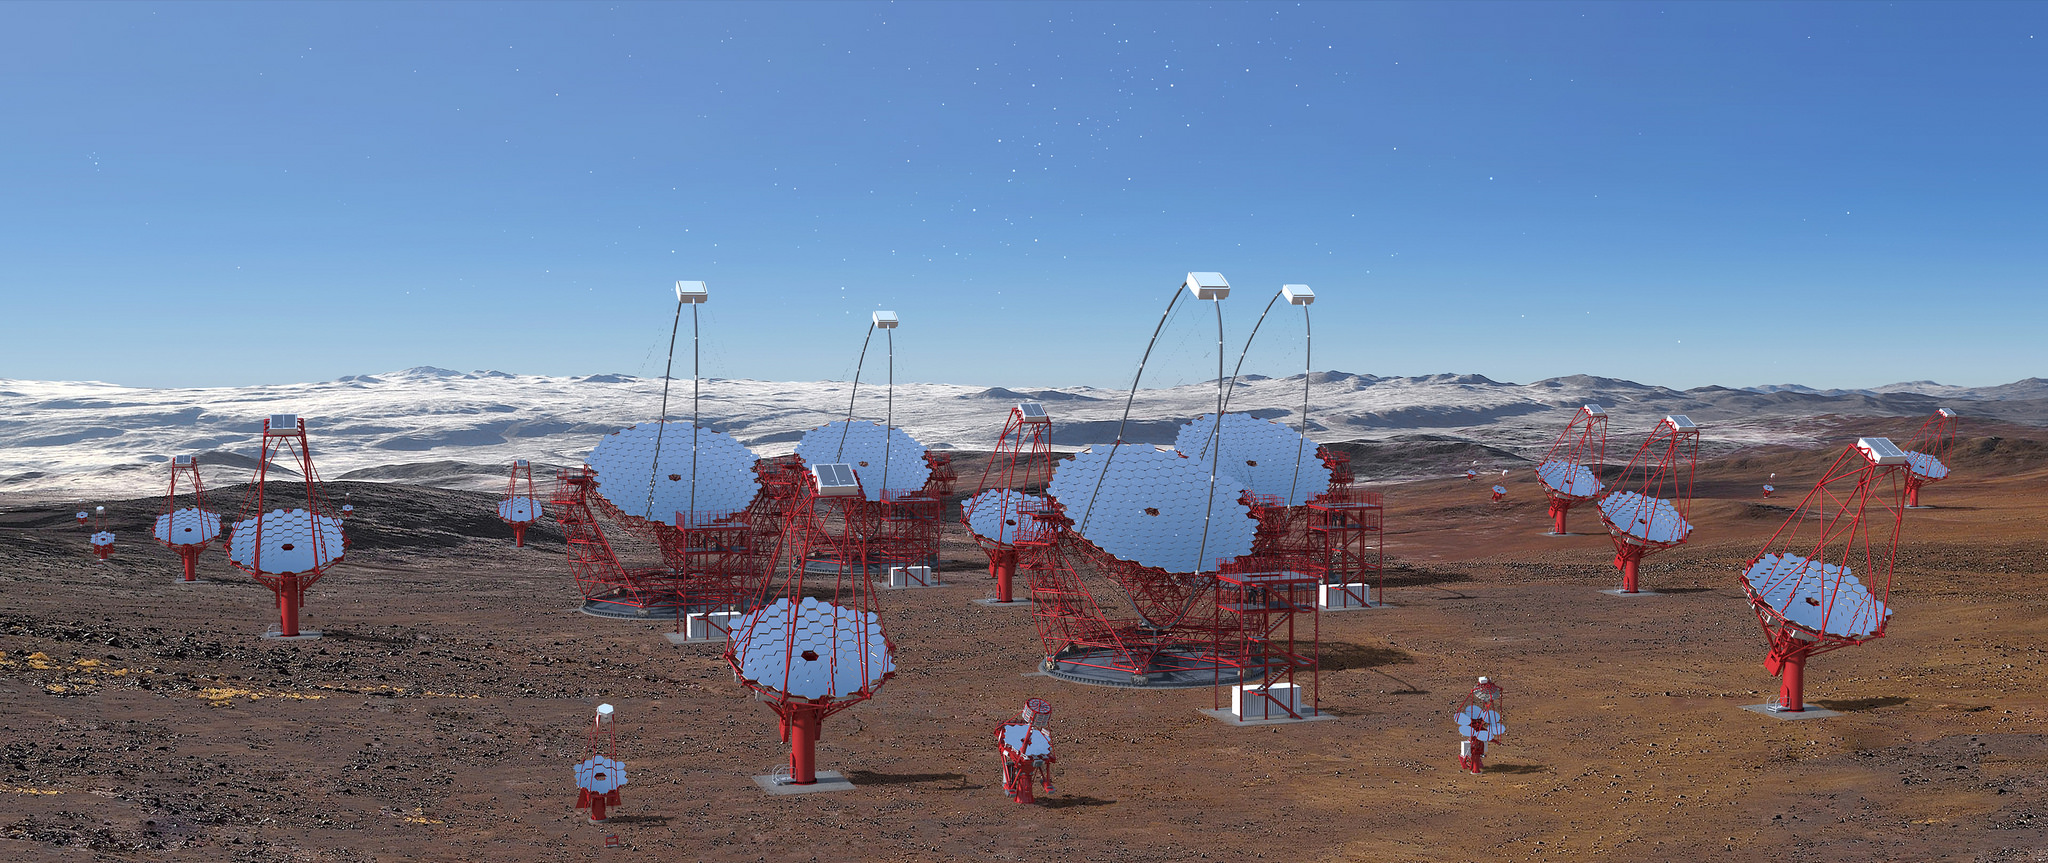
\includegraphics[width=14cm]{fig/CTA.jpg}
  % 図の説明が長い場合、[]で囲むことで短い図の説明を目次のみに表示できます。
  \caption[CTAの完成想像図]{CTAの完成想像図(画像提供:G.~Pérez、IAC、SMM)。JPEG(ビットマップ画像)なので、出力PDFで拡大するとドットが見えます。}
  % これで本文中から参照できます。
  \label{fig_CTA}
\end{figure}

\begin{figure}
  \centering
  % PDFも使えます。
  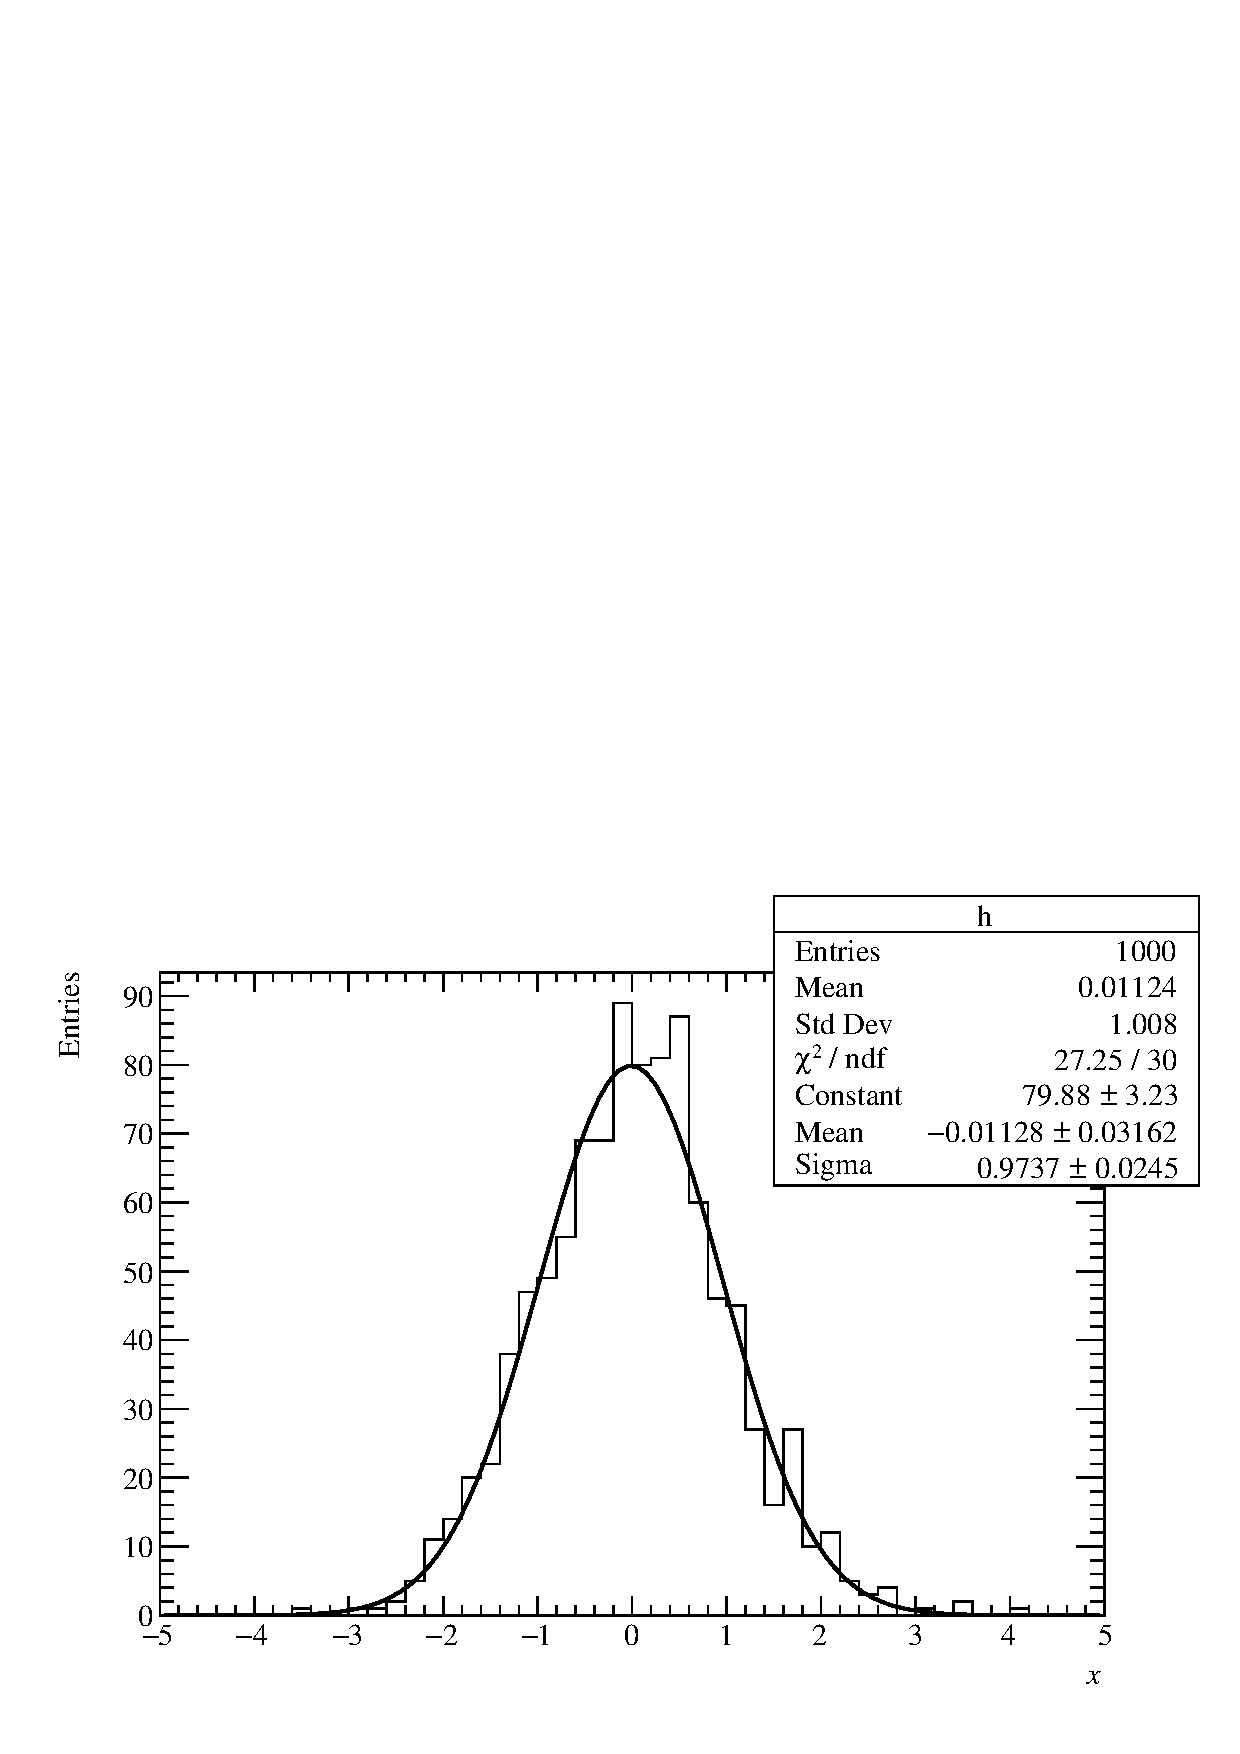
\includegraphics[width=14cm]{fig/histogram.pdf}
  \caption[ガウシアンでヒストグラムをフィットした例]{ガウシアンでヒストグラムをフィットした例。PDF(ベクター画像)なので、出力PDFで拡大しても滑らかです。また文字列もPDF中で検索することができます。}
  \label{fig_histogram}
\end{figure}

図を文中で参照したいときは\texttt{ref}コマンドを使用して、「図~\ref{fig_CTA}」のようにすることができます。この部分は\LaTeX{}中で実際には\texttt{図\~{}\bs{}ref\{fig\_CTA\}}と書いています。「図」と\texttt{\bs{}ref}の間に\texttt{\~{}}を入れるのは、「図」と図番号の間で改行を防ぐためです\footnote{このようにチルダを入れる手法は、人名の姓名の間や数値と単位の間で改行を防ぐのにも広く使われます。}。

\texttt{figure}環境で図を挿入する場所は、初めてその図を言及する段落の直後、もしくは直前です。あまりに離れた場所に図を挿入すると読者はどこに図があるかを探さなくてはならず、読むのが困難になるからです。

場合によっては複数の図を並べたいこともあるでしょう。そのようなときは、\texttt{subfigure}環境を使って図~\ref{fig_subfigure}のようにすることができます。\texttt{minipage}環境でも似たようなことができますが、\texttt{subfigure}を使うと小番号を自動で付与したり、「図~\ref{fig_subfigure_b}」のように、小番号を参照することができます。

\begin{figure}
  \centering
  \subfigure[]{% {の直後に%を置くことで、改行をさせない(図(b)を改行させない)。
    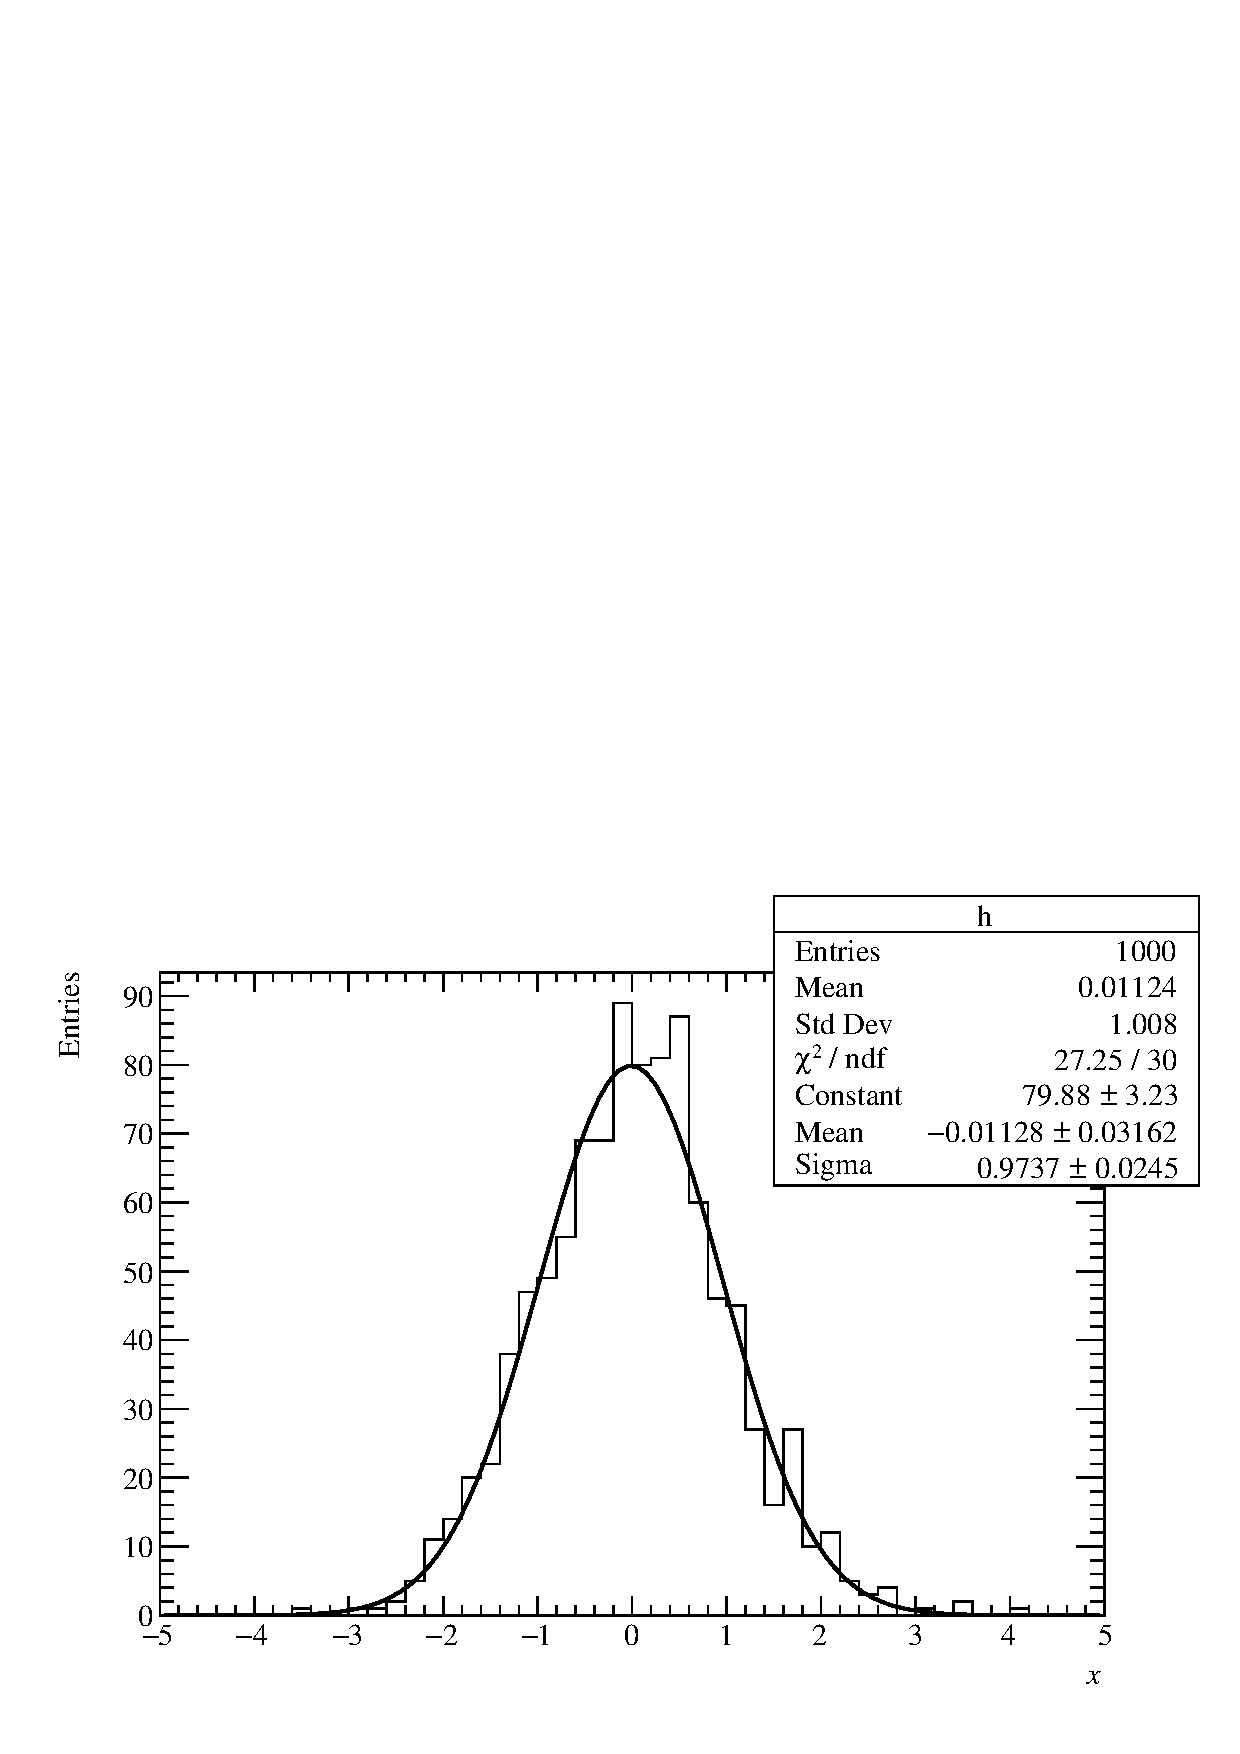
\includegraphics[width=.5\textwidth,clip]{fig/histogram.pdf}%
    \label{fig_subfigure_a}%
  }%
  \subfigure[]{%
    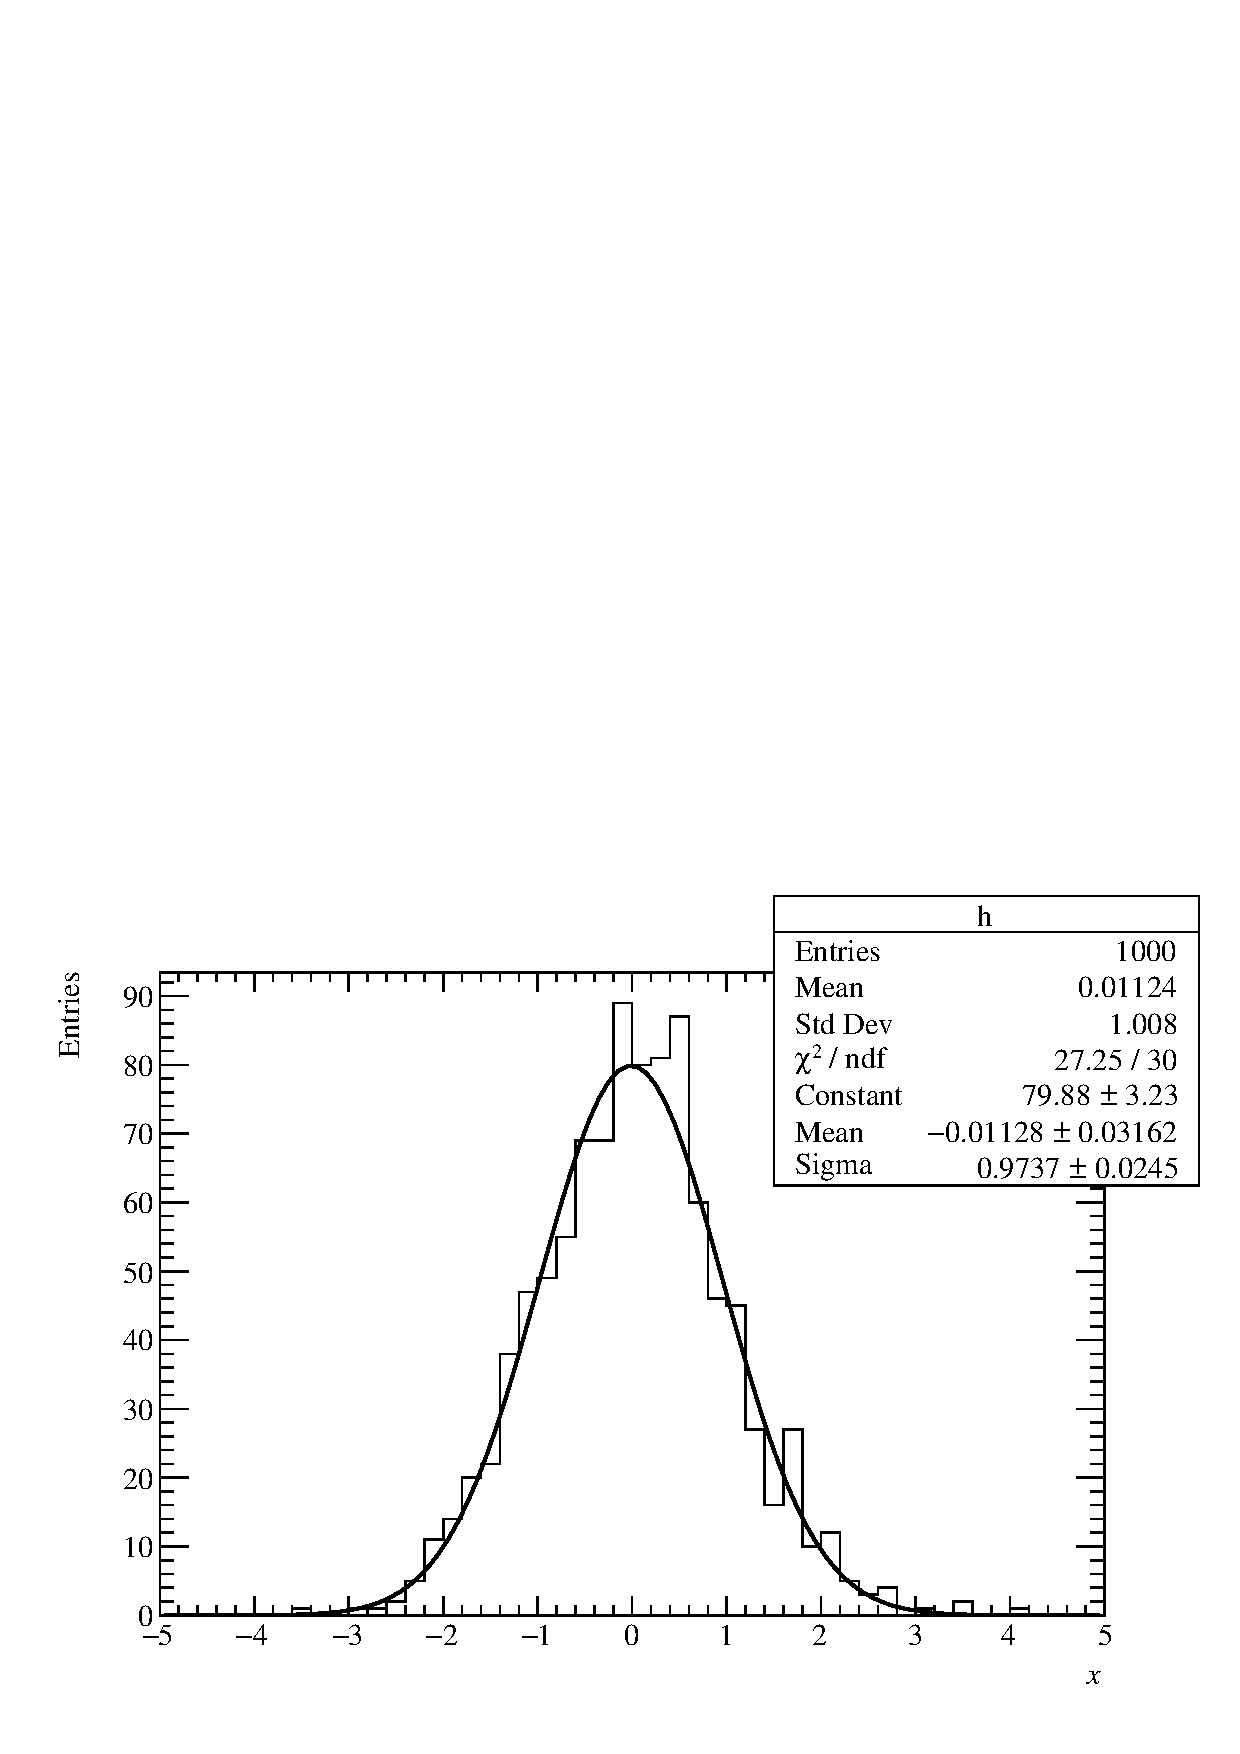
\includegraphics[width=.5\textwidth,clip]{fig/histogram.pdf}%
    \label{fig_subfigure_b}%
  }
  \subfigure[]{%
    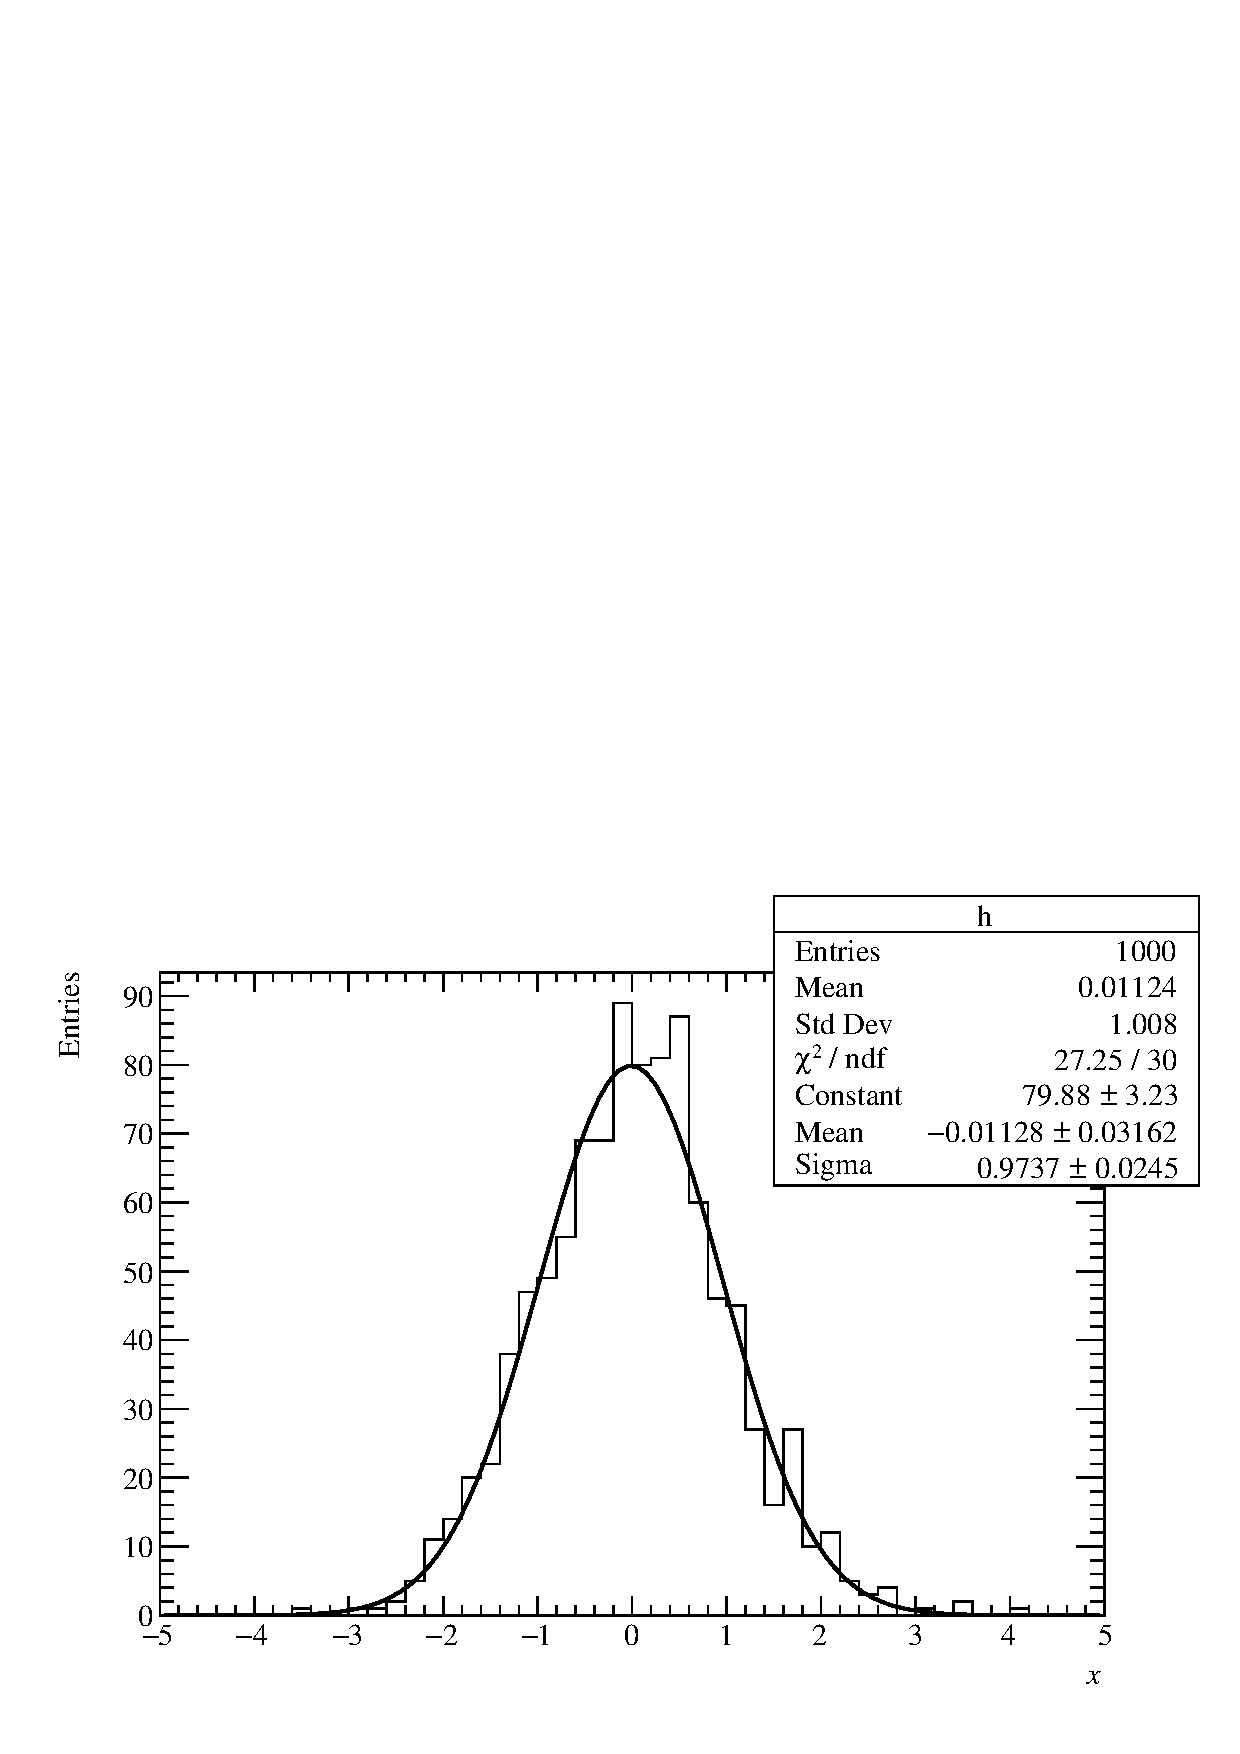
\includegraphics[width=.5\textwidth,clip]{fig/histogram.pdf}%
    \label{fig_subfigure_c}%
  }%
  \subfigure[]{%
    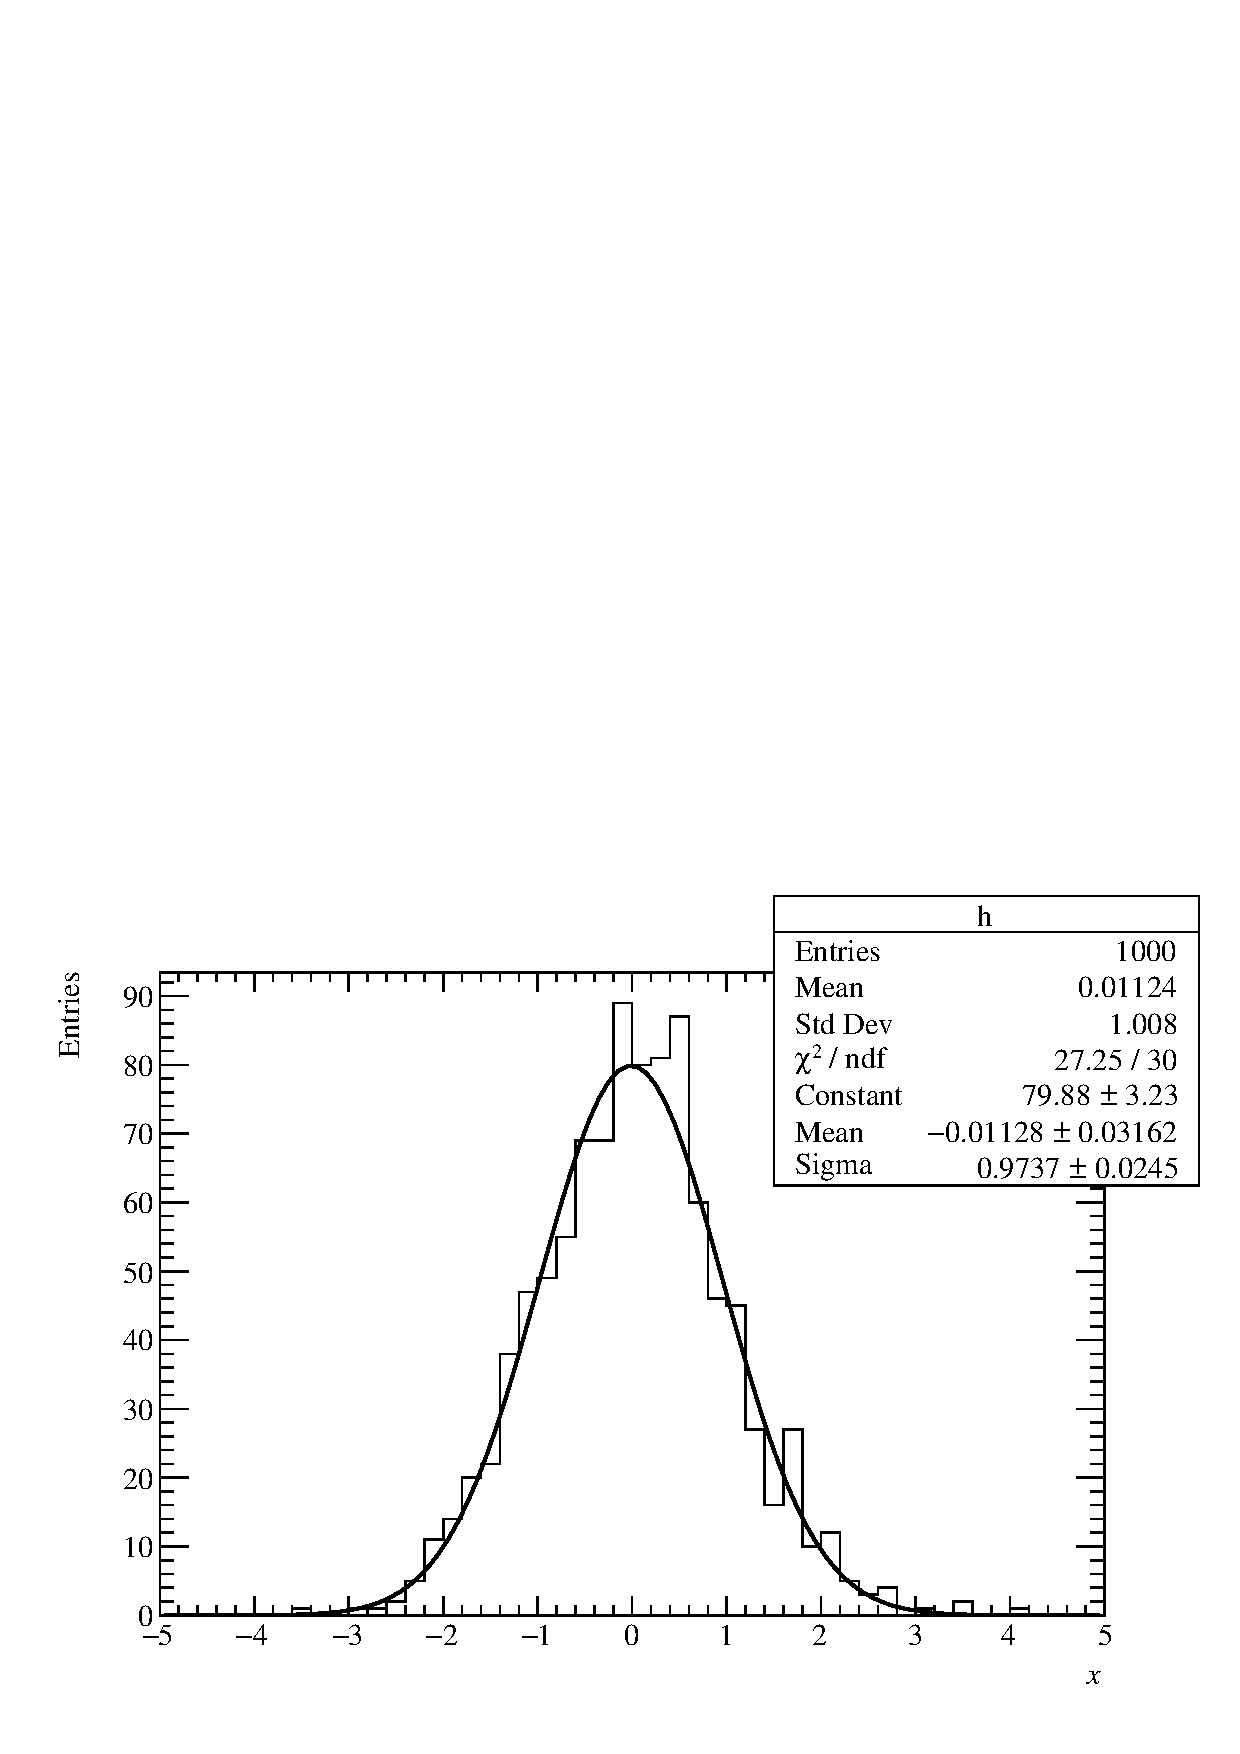
\includegraphics[width=.5\textwidth,clip]{fig/histogram.pdf}%
    \label{fig_subfigure_d}%
  }
  \caption[複数の図を並べた例]{複数の図を並べた例。(a)ガウシアンフィット。(b)同じもの。(c)これも同じもの。(d)これも同じもの。}
\label{fig_subfigure}
\end{figure}

またせっかく図の並べ方が分かったので、同じ図をPDF、PNG、JPEGにして図~\ref{fig_formats}にて比較してみましょう。それぞれの画像の特徴が分かります。また図~\ref{fig_formats}は参考のため\texttt{subfigure}ではなく\texttt{minipage}環境を使って作ってあります。

\begin{figure}
  \begin{minipage}[b]{.3333\linewidth}
    \leftline{(a)}
    \centering
    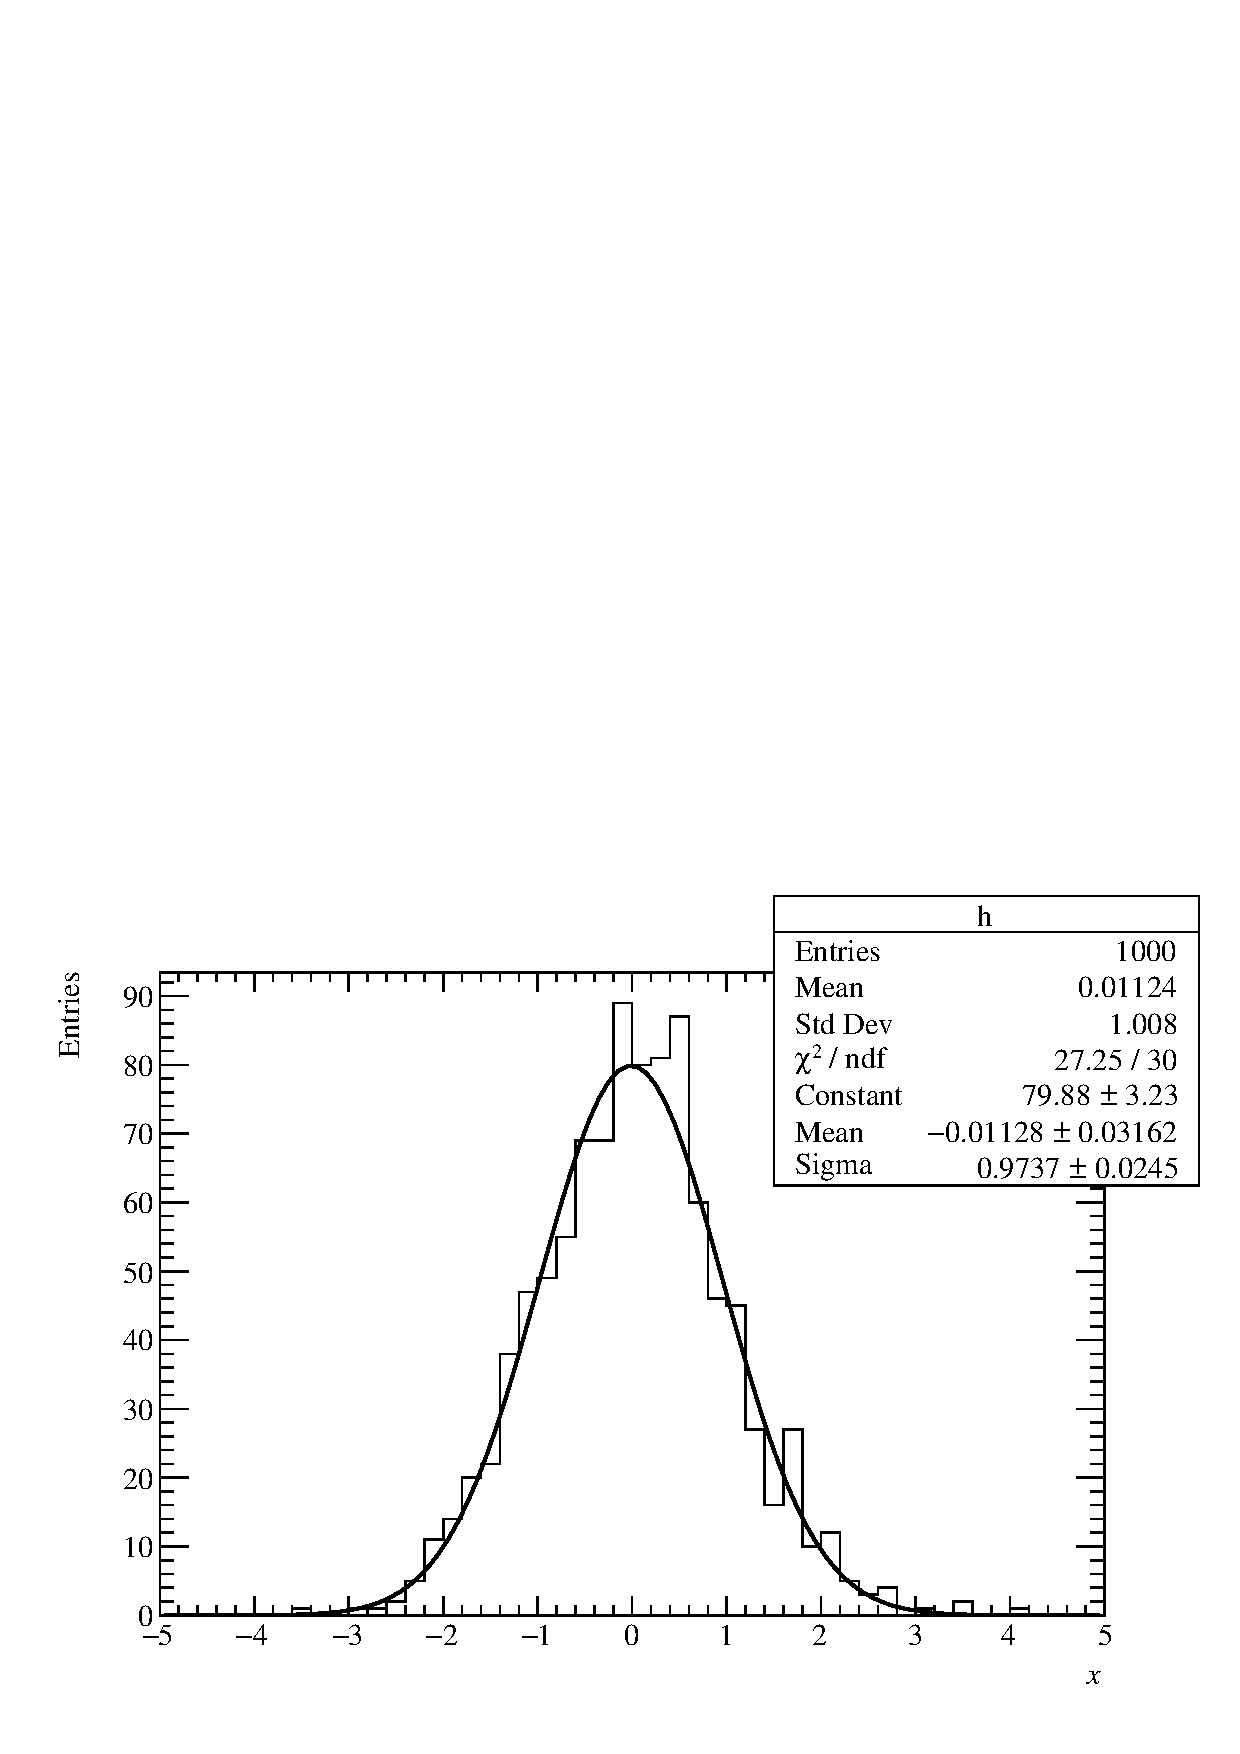
\includegraphics[width=5.5cm]{fig/histogram.pdf}
  \end{minipage}%
  \begin{minipage}[b]{.3333\linewidth}
    \leftline{(b)}
    \centering
    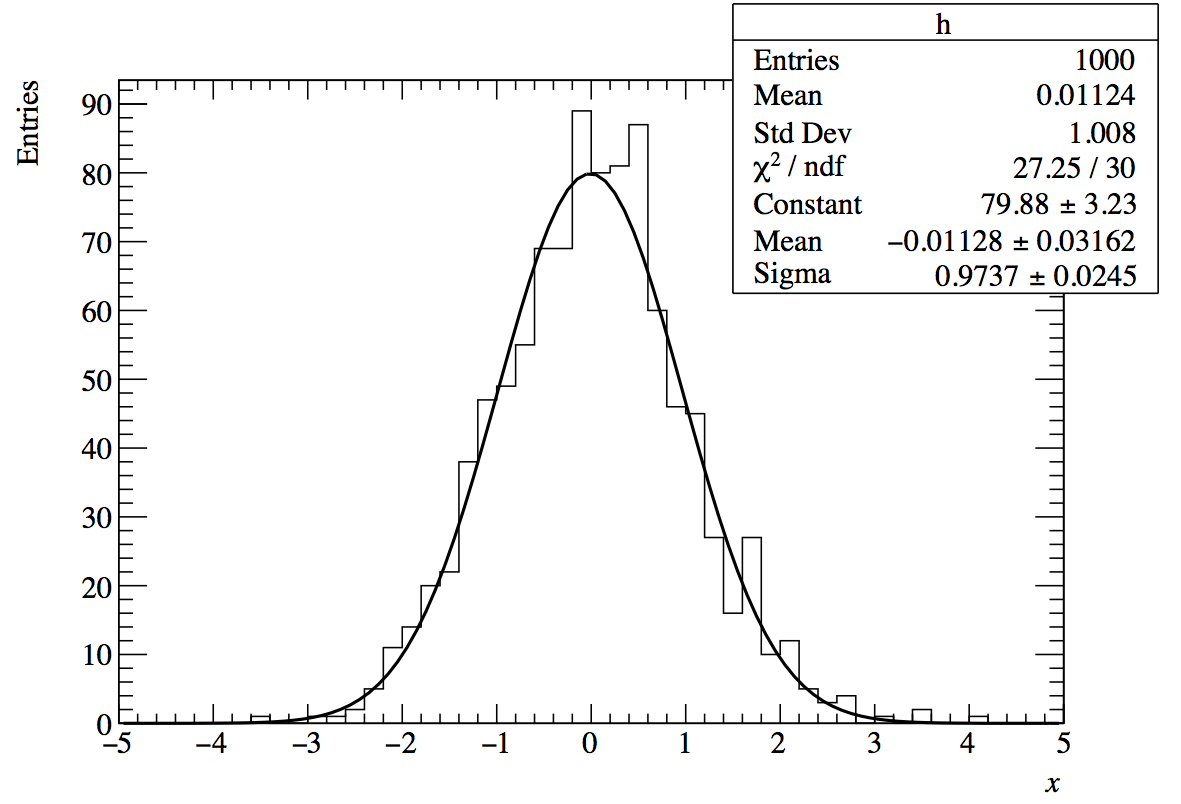
\includegraphics[width=5.5cm]{fig/histogram.png}
  \end{minipage}%
  \begin{minipage}[b]{.3333\linewidth}
    \leftline{(c)}
    \centering
    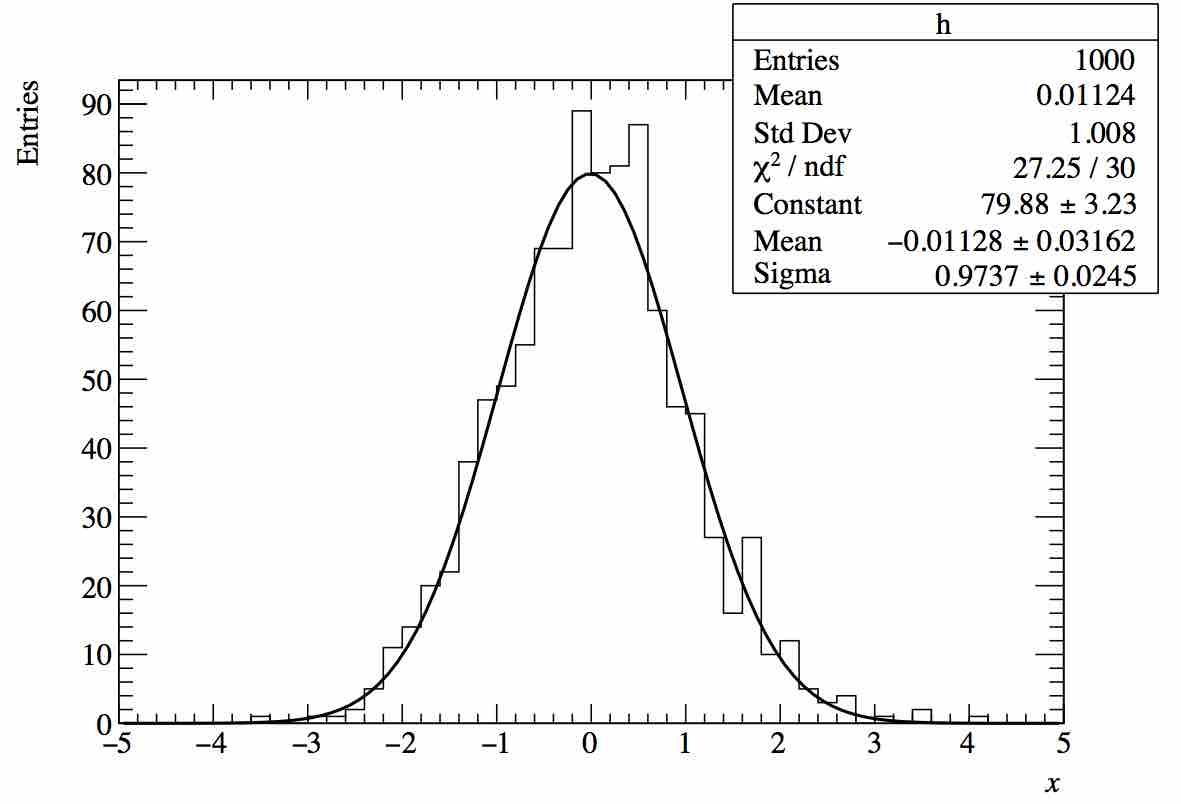
\includegraphics[width=5.5cm]{fig/histogram.jpg}
  \end{minipage}
  \caption[異なる画像形式の比較]{異なる画像形式の比較。(a) PDF形式。拡大しても綺麗であり、文字も検索やコピーができる。(b) PNG形式。拡大するとビットマップ画像であることが分かる。文字を選択できない。(c) JPEG形式。PNGに比べ、JPEG圧縮特有のブロックノイズ、モスキートノイズが発生しており非常に汚いことが分かる。}
  \label{fig_formats}
\end{figure}

\section{表の使い方}

表~\ref{tab_cta}に、\LaTeX{}でどのように表を作成するかの例を示します。実際にどういう \LaTeX{}コードがこの表に対応するのかは、ファイルの中身を眺めてください。

\begin{table} % 表も[htbp]のような場所指定は特に必要ない
  \centering
  % 表のキャプションは必ずその表の上に来ます。図の場合は下です。違いに気をつけてください。
  \caption{CTA で使用される望遠鏡の性能諸元}
  \footnotesize % 横幅のある表なので、文字サイズを小さくしています。通常は必要ありません。
  \label{tab_cta} % ラベルのつけ方は図と同様です。
  \begin{tabular}{lccccccc} % 列が何列あるかを示します。lcrはそれぞれ左・中央・右揃えの指定です。
    \hline
    &
    \shortstack{大口径望遠鏡 \\ Large-Sized Telescope \\ (LST)} &
    % 複数列を結合したいときは、multicolumnを使います。
    \multicolumn{2}{c}{\shortstack{中口径望遠鏡 \\ Medium-Sized Telescope \\ (MST)}} &
    \shortstack{SC 中口径望遠鏡 \\ Schwarzschild--Couder MST \\ (SC-MST)} &
    \multicolumn{3}{c}{\shortstack{小口径望遠鏡 \\ Smalle-Sized Telescope \\ (SST)}} \\
    & & FlashCam & NectarCAM & & GCT & ASTRI & 1M-SST \\
    \hline
    エネルギー範囲 & 20--200 GeV & \multicolumn{2}{c}{100 GeV -- 10 TeV} & 200 GeV -- 10 TeV & \multicolumn{3}{c}{5--300 TeV} \\
台数(北半球)& 4 & \multicolumn{2}{c}{15} & 0 & \multicolumn{3}{c}{0} \\
台数(南半球)& 4 & \multicolumn{2}{c}{24} & 24 & \multicolumn{3}{c}{70--90} \\
鏡直径 &	23~m & \multicolumn{2}{c}{12~m} & 9.7~m & 4~m & 4~m & 4~m \\
焦点距離 & 28~m & \multicolumn{2}{c}{16~m} & 5.6~m & 2.3~m & 2.15~m & 5.6~m \\
視野 & 4.5$^\circ$ & \multicolumn{2}{c}{7.7$^\circ$} & 8$^\circ$ & 8.6$^\circ$ & 9.6$^\circ$ & 9$^\circ$ \\
光学系 & 放物鏡 & \multicolumn{2}{c}{Davies--Cotton (DC)} & Schwarzschild--Couder (SC) & SC & SC & DC \\
画素数 & 1,855 & 1,764 & 1,855 & 11,328 & 2,048 & 1,984 & 1,296\\
\hline
  \end{tabular}
  \normalsize % 文字サイズを元に戻します
\end{table}

論文中で使う表の一般的な注意点として、あまり罫線をたくさん使いすぎないことです。日本では全てのセルの周辺に罫線を使う傾向があり、最悪、表~\ref{tab_cta_bad}のようになります。窮屈になるので、このような罫線の多用はやめましょう。

\begin{table}
  \centering
  \caption{表~\ref{tab_cta}の悪い例}
  \footnotesize
  \label{tab_cta_bad}
  \begin{tabular}{|l|c|cc|c|ccc|}
    \hline
    &
    \shortstack{大口径望遠鏡 \\ Large-Sized Telescope \\ (LST)} &
    % 複数列を結合したいときは、multicolumnを使います。
    \multicolumn{2}{c|}{\shortstack{中口径望遠鏡 \\ Medium-Sized Telescope \\ (MST)}} &
    \shortstack{SC 中口径望遠鏡 \\ Schwarzschild--Couder MST \\ (SC-MST)} &
    \multicolumn{3}{c|}{\shortstack{小口径望遠鏡 \\ Smalle-Sized Telescope \\ (SST)}} \\
    \hline
    & & FlashCam & NectarCAM & & GCT & ASTRI & 1M-SST \\
    \hline
    エネルギー範囲 & 20--200 GeV & \multicolumn{2}{c|}{100 GeV -- 10 TeV} & 200 GeV -- 10 TeV & \multicolumn{3}{c|}{5--300 TeV} \\
    \hline
    台数(北半球)& 4 & \multicolumn{2}{c|}{15} & 0 & \multicolumn{3}{c|}{0} \\
    \hline
    台数(南半球)& 4 & \multicolumn{2}{c|}{24} & 24 & \multicolumn{3}{c|}{70--90} \\
    \hline
    鏡直径 &	23~m & \multicolumn{2}{c|}{12~m} & 9.7~m & 4~m & 4~m & 4~m \\
    \hline
    焦点距離 & 28~m & \multicolumn{2}{c|}{16~m} & 5.6~m & 2.3~m & 2.15~m & 5.6~m \\
    \hline
    視野 & 4.5$^\circ$ & \multicolumn{2}{c|}{7.7$^\circ$} & 8$^\circ$ & 8.6$^\circ$ & 9.6$^\circ$ & 9$^\circ$ \\
    \hline
    光学系 & 放物鏡 & \multicolumn{2}{c|}{Davies--Cotton (DC)} & Schwarzschild--Couder (SC) & SC & SC & DC \\
    \hline
    画素数 & 1,855 & 1,764 & 1,855 & 11,328 & 2,048 & 1,984 & 1,296\\
    \hline
  \end{tabular}
  \normalsize % 文字サイズを元に戻します
\end{table}

\section{数式の使い方}

\LaTeX{}を使う理由のひとつが、数式を綺麗に出力できるというのがあります。例えば中性パイ中間子$\pi^0$のガンマ線への二体崩壊であれば
\begin{equation}
  \pi^0 \rightarrow \gamma + \gamma
\end{equation}
のように書けますし、もっとややこしい数式も色々と書けますが、詳細は「LaTeX 数式」などでインターネット上で検索してください。この例のように、本文中に数式を入れるときは\texttt{\$\$}でその式を囲み、独立した行に数式を書くときは\texttt{equation}や\texttt{align}\footnote{\texttt{amsmath}パッケージで使用可能です。}環境を使ってください。

\subsection{斜体と立体}
数式を書くときには「斜体」(italic)と「立体」(upright)の違いに気をつけてください。基本的に数式は斜体を使って書きます。何も考えずに\LaTeX{}を使えば全て斜体になります。

ただし、次の2つの式を見比べてみてください。
\begin{equation}
  e^{ix}=cosx + isinx
  \label{eq_italic}
\end{equation}
\begin{equation}
  \mathrm{e}^{\mathrm{i}x}=\cos x + \mathrm{i}\sin x
  \label{eq_upright}
\end{equation}
式~\ref{eq_italic}は全ての文字が斜体で書かれていますが、式~\ref{eq_upright}は$x$以外は立体です。このように、いくつかの文字では立体を使うのが一般的です。例えば$\log$、$\sin$、$\mathrm{e}$(自然対数の底)、$\mathrm{i}$(虚数単位)、$\mathrm{d}$(微分作用素)などは、それぞれ\texttt{\bs{}log}、\texttt{\bs{}sin}、\texttt{\bs{}mathrm\{e\}}、\texttt{\bs{}mathrm\{i\}}、\texttt{\bs{}mathrm\{d\}}などと入力することで書くことができます\footnote{自然対数の底や虚数単位の場合は、分野や国によって斜体にするかどうかの違いがあります。また微分作用素は斜体で$d$とする場合もありますが、立体にすることで長さを表すのに頻繁に使われる変数$d$と区別する効果があります。}。

ここで\texttt{\bs{}mathrm}というコマンドが出てきましたが、これは数式中で文字を立体にするためのコマンドです。特定の文字を立体にするときだけでなく、変数名の添字を立体するときにも使います。例えばトリガー回数を示す変数は$N_\mathrm{trigger}$などと書くことがあると思いますが、このときに「trigger」の部分は変数ではありませんので、斜体にしません。

\subsection{単位}
数式中に単位を使うとき、\texttt{\bs{}mathrm}を使わずに$100 MeV$などとしてしまう間違いもよく見られます。このように斜体になったものは変数$M$と$e$と$V$の掛け算であり、単位ではありません。また100MeVのように単位と数値の間にスペースのない書き方をする人も見かけますが、これも間違いです。本文中に書くときは\texttt{100\~{}MeV}とし、\texttt{equation}環境中では\texttt{100\bs{} \bs{}mathrm\{MeV\}}と書きます\footnote{余計なバックスラッシュとスペースは、数字と単位の間にスペースを入れるためです。}。

\LaTeX{}では\texttt{\%}の後ろをコメントとして扱いますので、95\%のようにパーセントの表示をしたい場合には\texttt{95\bs{}\%}のように書きます。\%と数値の間にスペースを入れるかどうかは、流派が2つありますが、私の周りでは入れない人が多いようです\footnote{入れない理由としては、\%は単位ではなく0.01という数だから、というものが挙げられます。}。

\section{引用の仕方}

研究や論文というのは過去に誰かのやった研究を前提として新たに何かを進歩させるためにあります\footnote{「巨人の肩の上に立つ」とよく表現されます。}。しかしあなたの修士論文に全ての過去の研究を書くことはできませんので、引用という形式を使い他の論文をその事実の出典とします。

ここで、「引用」と日本語で書いた場合には「quotation」と「citation」の2つの英語に翻訳され得ますが、我々の論文で通常用いるのは「citation」のほうです。著作権法などで問題になるのは「quotation」のほうなので、間違えないようにしてください。

\LaTeX{}で\texttt{citep}コマンドや\texttt{citet}コマンドを使って論文を引用(cite)するときは、例えば次のようになります。

\begin{quote} % ここで LaTeX の体裁を整えるために quote コマンドを使っていますが、ここは「引用」(quote)しているわけではりません。
  宇宙線の全粒子スペクトルは図 XX に示すように$10^9$~eVから$10^{20}$~eVまでおよそ$-3$乗の冪で減少している\citep{Swordy2001}。$10^{12}$~eV(1~TeV)付近のガンマ線は超高エネルギーガンマ線と呼ばれ、様々な観測手法が提案されている\citep[例えば][を見よ]{Okumura2005}。この\citet{Okumura2005}の手法では\ldots
% 複数の文献を一度に引用するには \citep{Swordy2001,Okumura2005}とすることもできます。
\end{quote}
ここでは引用(cite)を3回しており、それぞれ\texttt{citep}、\texttt{citep}、\texttt{citet}コマンドを使っています。

\section{\BibTeX{}の使用}
このテンプレートの場合、\pageref{page:bib}ページに「引用文献」という箇所があります。このページを手作業で間違いなく整形するのは面倒です。手でやる代わりに\BibTeX{}という仕組みを使います。\texttt{thesis.bib}というファイルに引用文献の必要な情報が書かれていますので、これを参考にして\BibTeX{}ファイルを作るか、論文をダウンロードするときに\texttt{.bib}ファイルもダウンロードできますので、それを使ってください\footnote{近年は「文献管理ソフト」と呼ばれるものが発達していますので、特に博士進学する学生は好きなものを入れてみてください。}。

\section{ヨーロッパ圏の人名など}
ウムラウトなどの混じったヨーロッパ圏の人名を入力するには、例えばシュレーディンガーの場合、\LaTeX{}では\texttt{Shr\bs{}"\{o\}dinger}と入力することでShr\"{o}dingerと表示すると\LaTeX{}の教科書には書いてあります。しかしいちいちこんなことをするのは面倒ですので、\texttt{main.tex}に書いてある\texttt{\bs{}usepackage[utf8]\{inputenc\}}を使うことで、直接ウムラウトつきの文字を\LaTeX{}のソース中に書いてしまって問題ありません。「ö」と「\"{o}」は、この\LaTeX{}ソース中では違う入力方法で書かれていますが、出力は同一です。

\section{\texttt{newcommand}}

入力が長く、論文中で何度も繰り返し使うような入力はコマンドとして登録することができます。例えば\texttt{\bs{}HI\{\}}や\texttt{\bs{}bs\{\}}といったコマンドを\texttt{main.tex}で定義しており、これらの結果は「\HI{}」や「\bs{}」と表示されます。

\chapter{剽窃について}

\section{剽窃とは何か}
\label{sec:plagiarism}
「剽窃(ひょうせつ)」とは
\begin{itemize}
\item 「他人の作品や論文を盗んで、自分のものとして発表すること。」『大辞泉』
\item 「他人の作品・学説などを自分のものとして発表すること。」『スーパー大辞林』
\item 「他人の著作から,部分的に文章,語句,筋,思想などを盗み,自作の中に自分のものとして用いること。他人の作品をそっくりそのまま自分のものと偽る盗用とは異なる。」『ブリタニカ国際大百科事典 小項目事典』
\end{itemize}
のように辞書では説明されています。

例えばここで『ブリタニカ国際大百科事典 小項目事典』を引用元として明記せずに、
\begin{quotation}
  \red{剽窃(ひょうせつ)とは、}他人の著作から\red{、}部分的に文章\red{、}語句\red{、}筋\red{、}思想などを盗み\red{、}自作の中に自分のものとして用いること\red{です}。他人の作品をそっくりそのまま自分のものと偽る盗用とは異な\red{ります}。
\end{quotation}
という説明をしたとします。これが剽窃です。この例では赤字で示したとおり、文体をですます調に変更したり、読点を「,」から「、」に変更したり、文頭に「剽窃(ひょうせつ)とは、」と書き加えたりしていますが、全体としては同一の文章であるため、通常は剽窃と見なされます。

学術論文ではない創作物の形態によっては、剽窃行為が「インスパイア」や「オマージュ」という言葉で括られることもあります。しかし修士論文での剽窃行為は不正行為です。試験でのカンニングやレポートの丸写しと同じであり、(まともな大学や研究室であれば)厳しく罰せられます。

\section{剽窃をするとどうなるか}

修士論文中に剽窃行為が発見された場合、その学期における単位をすべて没収され、卒業に必要な単位が与えられず修士課程を修了できなくなる可能性が高いです。各大学や研究科でどのような対応を実際に取るかはそれぞれだと思いますが、少なくとも私が審査員を担当した場合には落第させます。

修論審査に落第すれば、もし就職が決まっていても留年を余儀なくされます。留年を選択せず修了を諦めて中退するにしても、就職先は剽窃行為のせいで修了できなかった学生をそのまま採用はしてくれないでしょう。仮に同じ企業に就職が認められたとしても、修士卒扱いで入社できたはずのところが学部卒扱いとなり、初任給が月額数万円低い状態から開始となります。例えば同期と2万円の月給差を保ったまま40 年間働くとすると生涯収入で 1000 万円程度の損失になります。もし留年する道を選んでも、定年時点で1000万円程度の年収を見込めるのであれば、生涯収入としてその額だけ失うことになります。

もし博士課程に進学する場合、なぜ留年したかの説明を陰に陽に常に求められます。たとえ直接にその理由を問われることがなくとも、他の学生より1年多く修士課程に時間がかかったということは、優秀な学生ではないと周りから見なされ、研究をする上でも奨学金などを取得する上でも不利になるでしょう。また標準年限を超えての在籍の場合、大学院の授業料免除などの制度も利用できなくなる可能性があります。

\section{修士論文における剽窃について}
節\ref{sec:plagiarism}に引用した一般的な剽窃の定義ではなく、科学文書や、特に修士論文での剽窃についてもう少し踏み込んで説明し直してみましょう。

\subsection{いわゆるコピペ}

少なくとも宇宙物理学分野における修士論文は独自性のあるものでなくてはいけません。独自性のある(オリジナル)とは次のようなことです。
\begin{itemize}
\item 誰かが過去にやった研究ではないこと
\item 自分自身の手でやった研究であること(共同研究であれば、十分に自分の貢献のあること)
\item 研究本体以外の章も含め、すべて自分の言葉で説明できること
\end{itemize}

したがって、誰かの論文や教科書の記述をそっくりそのまま持ってきて(いわゆる「コピペ」して)、それを自分の修士論文として提出することは許されません。高校や大学のレポートなどでも、他人のレポートを写すなと散々注意されるのと同じことです。

これはコピペする文章の長さに依りません。たとえ1行であってもコピペはコピペであり、剽窃と見なされます\footnote{ただし、ごくありふれた表現や、酷似するのが避けられない科学的事実は除く。}。

もちろん、ある文章を他の論文や書籍から引用(quote)する必要のある場合は、逆に改変してはいけません。そっくりそのまま書き写し、それを自分の文章とは別のものであると分かるように引用符や枠で囲むなりします。しかし宇宙物理学関連の修士論文でこのような引用をすることは、ほとんどないと思います。

\subsection{他人の文章の改変}

コピペとともによく見られるのが、他人の文章を一部だけ改変して自分が書いたかのように装うことです。完全に同一のものを持ってくる方が簡単ですし、なぜこのような行動を取るのかよく分かりませんが、私の経験として最も多い剽窃行為がこの文章の一部改変です。

もしかすると「先輩の修論を写したりコピペするなよ。自分の言葉で書けよ」とだけ教員から指導を受けると、表面的に一部改変すれば剽窃にはならないと勘違いするのかもしれません。しかし元の文章が存在しなければ作成できないのですから、これは独自性のある文章とは見なされず、やはり剽窃行為となります。

たとえば次のような文章が「元ネタ」として存在していたとしましょう\footnote{これはきちんと添削を受けていない、今となっては恥ずかしい私の修論の一節ですが、あくまで例です。}。

\begin{quotation}
  1910年代にHessらによって宇宙線の存在が確認されて以来、様々なエネルギー領域、様々な検出器によって宇宙線の観測が行われてきた。同時に、ガリレオ以来発達してきた可視光による天体の観測も、電波望遠鏡や赤外望遠鏡の登場によって多波長での観測へと発展することとなった。

  宇宙線と言っても、その成分は電磁波、陽子、原子核、neutrinoなど様々であり、それらの持つエネルギーも広範にわたる。現在地球上で確認されている宇宙線のうち、最もエネルギーの高いものは$10^{20}$~eVを超える(最高エネルギー宇宙線)。これは人工的に到達できるエネルギーを実に8桁も上回るが、なぜそのような高エネルギーの宇宙線が存在するのかは謎である。加速機構、地球までの伝播過程、1次宇宙線成分は何であるのか、いずれも未解明のままであり、その興味は尽きない。
  \flushright{\citet{Okumura2005}より引用}
\end{quotation}

少しこれを改変してみましょう。赤字が削除箇所、青字が追加箇所です。実際に私が発見してきた剽窃行為には、このような改変が多くありました。
  
\begin{quotation}
\DIFdelbegin \DIFdel{1910年}\DIFdelend \DIFaddbegin \DIFadd{1912}\DIFaddend \DIFdelbegin \DIFdel{代}\DIFdelend \DIFaddbegin \DIFadd{年}\DIFaddend に\DIFaddbegin \DIFaddend Hess\DIFdelbegin \DIFdel{ら}\DIFdelend によって宇宙線\DIFdelbegin \DIFdel{の存在}\DIFdelend が\DIFdelbegin \DIFdel{確認}\DIFdelend \DIFaddbegin \DIFadd{初めて発見}\DIFaddend されて以来、\DIFdelbegin \DIFdel{様々な}\DIFdelend \DIFaddbegin \DIFadd{広い}\DIFaddend エネルギー\DIFdelbegin \DIFdel{領域}\DIFdelend \DIFaddbegin \DIFadd{範囲}\DIFaddend 、\DIFdelbegin \DIFdel{様々}\DIFdelend \DIFaddbegin \DIFadd{多種多様}\DIFaddend な検出器によって宇宙線\DIFdelbegin \DIFdel{の}\DIFdelend \DIFaddbegin \DIFaddend 観測が行われてきた。\DIFdelbegin \DIFdel{同時に}\DIFdelend \DIFaddbegin \DIFadd{また}\DIFaddend 、ガリレオ以来発達してきた可視光\DIFdelbegin \DIFdel{による天体の観測}\DIFdelend \DIFaddbegin \DIFadd{での天体観測}\DIFaddend も、電波望遠鏡や赤外望遠鏡\DIFaddbegin \DIFadd{という新しい観測手段}\DIFaddend の登場\DIFdelbegin \DIFdel{によって多波長での観測}\DIFdelend \DIFaddbegin \DIFadd{により、多波長観測}\DIFaddend へと発展\DIFdelbegin \DIFdel{することとなった}\DIFdelend \DIFaddbegin \DIFadd{した}\DIFaddend 。

宇宙線と\DIFdelbegin \DIFdel{言}\DIFdelend \DIFaddbegin \DIFadd{い}\DIFaddend っても、その成分は\DIFdelbegin \DIFdel{電磁波、}\DIFdelend 陽子、原子核、\DIFdelbegin \DIFdel{neutrino}\DIFdelend \DIFaddbegin \DIFadd{電子、ニュートリノ}\DIFaddend など様々であり、\DIFdelbegin \DIFdel{それらの持つ}\DIFdelend \DIFaddbegin \DIFadd{その}\DIFaddend エネルギー\DIFaddbegin \DIFadd{範囲}\DIFaddend も\DIFdelbegin \DIFdel{広範}\DIFdelend \DIFaddbegin \DIFadd{何桁}\DIFaddend に\DIFaddbegin \DIFadd{も}\DIFaddend わたる。現在\DIFdelbegin \DIFdelend \DIFaddbegin \DIFadd{、}\DIFaddend 地\DIFdelbegin \DIFdel{球}\DIFdelend 上で確認されている宇宙線のうち、最もエネルギーの高いものは$10^{20}$~eVを超える(\DIFaddbegin \DIFadd{いわゆる}\DIFaddend 最高エネルギー宇宙線)。これは\DIFdelbegin \DIFdel{人工的に}\DIFdelend \DIFaddbegin \DIFadd{加速器で人類が}\DIFaddend 到達できるエネルギーを\DIFdelbegin \DIFdel{実に}\DIFdelend 8桁も上回るが、なぜそのような高\DIFaddbegin \DIFadd{い}\DIFaddend エネルギーの宇宙線が存在するのかは\DIFdelbegin \DIFdel{謎である}\DIFdelend \DIFaddbegin \DIFadd{解明されていない}\DIFaddend 。\DIFaddbegin \DIFadd{宇宙線の}\DIFaddend 加速機構、地球までの伝播過程、\DIFaddbegin \DIFadd{また}\DIFaddend 1次宇宙線成分は何であるのか\DIFaddbegin \DIFadd{は}\DIFaddend 、いずれも未解\DIFdelbegin \DIFdel{明}\DIFdelend \DIFaddbegin \DIFadd{決}\DIFaddend の\DIFdelbegin \DIFdel{まま}\DIFdelend \DIFaddbegin \DIFadd{問題}\DIFaddend であり、\DIFdelbegin \DIFdel{その興味は尽きない}\DIFdelend \DIFaddbegin \DIFadd{将来の宇宙線観測計画による解決が期待される}\DIFaddend 。
  \flushright{\citet{Okumura2005}を意図的に改変}
\end{quotation}

\subsection{元の文章を下敷きに自分で考えたつもりになったもの}

さらに改変の量を増やし、ところどころに自分の独自の文を入れたり、文の前後を入れ替える剽窃もあります。自分で考えて文を挿入するのだから剽窃ではないと考える人もいるかもしれませんが、やはり元の文章が存在しなければ書くことのできない文章ですので、これも立派な剽窃です。たとえば次のようなものです。

\begin{quotation}
  Hessの気球実験によって1912年に宇宙線が大気中で発見されてから、様々な粒子、多様な検出手法、またMeV領域から$10^{20}$~eVにまでおよぶエネルギー範囲で宇宙線の観測が行われてきた。一方、電磁波による天体の観測も、ガリレオによる可視光観測に始まり、電波望遠鏡や赤外線望遠鏡などの登場によって他波長観測へと発展した。さらに近年の重力波やニュートリノ観測を加え、現在の宇宙観測は、多粒子、他波長観測の時代、すなわちマルチメッセンジャー天文学へと進展した。

  このうち宇宙線は、陽子、原子核、電子、ニュートリノなどを含む、宇宙空間を飛び交う高エネルギーの粒子である。先に述べたように、その最高エネルギーは$10^{20}$~eVにまでわたる(いわゆる最高エネルギー宇宙線)。これは人類がLHC加速器で到達できる数~TeVというエネルギーを8桁も上回るものであるが、なぜそのような高いエネルギーの宇宙線が宇宙で加速されているのか、宇宙線の発見から100年以上が経っても未解決の問題である。その加速機構、加速天体、地球までの伝播、また粒子の種類がなんであるかという謎を解き明かすには、今後の宇宙線観測手法に大きな飛躍が必要である。
  \flushright{\citet{Okumura2005}を意図的に改変}
\end{quotation}

ここまで改変すると、全く違う文章のように感じる人もいるかもしれませんが、実際に行われる剽窃行為では、このような元ネタに改変を加えた文章が何段落も続くことが多いです。そのため、文章の一部が似通っているだけでなく、その章の論理展開自体がほとんど同じになってしまうのです。

研究背景は過去に行われた研究の積み重ねなので、論理展開が同じになることは仕方がないという主張をする学生もいます。しかし修士論文はその研究目的が各々違うわけですから、論文のイントロなどで全く同じ論理展開になることは本来ありえません。その論文独自の研究内容を説明するためにイントロは書かれるべきであり、他の文章と同じであるというのは、イントロを書くという目的を勘違いしています。

\subsection{出典のない図表の使用}

他人の文章を剽窃する行為とは別に、図表を適切に引用(cite)せずに流用するという剽窃もあります。これは悪意があって行われているわけではなく、引用の作法を知らないだけの場合が多いため罪としては軽いかもしれません。しかし、その修士論文の読者に対して「この図は自分が作りました」と嘘をつくのと同じ行為ですので、やはり問題行為であることは理解できると思います。

このような図表の剽窃は、特に共同研究で多く見られます。ある実験プロジェクトに参加している場合、実験装置の説明の図や写真をプロジェクト内で使いまわすことがあるでしょう。たとえば図\ref{fig_CTA}のようなものが該当します。もしこれを出典もしくは作者を明記せずに使用した場合、剽窃行為に当たります\footnote{おそらく「出典を明記して再提出しろ」と言われるだけで、落第はしないと思いますが。}。

図表の提供者の名前を入れる、その図が最初に使われた論文や出版物が存在する場合はそれを出典として明記する(cite する)、もしくは提供した実験グループなどの名前を入れるなどしてください。

\subsection{アイデアの盗用}
他人の考えた研究アイデアを自分が考えたかのように記述するのも剽窃です。例えば投稿論文になっていないものの、先輩の修士論文で先行研究が行われていたとしましょう。これを先行研究として取り上げることなく、「〜〜という手法を本論文では考案し」などと書くのは剽窃行為です。きちんと「〜〜という手法が先行研究で提案され、本論文ではこれを発展させ」のように書きましょう。

\subsection{自己剽窃}

自己剽窃とは、自分の書いた論文などから図や文章を剽窃して再利用することです。なぜこれが問題とされるのか、直感的にはすぐに分からないかもしれません。

自己剽窃が最も問題とされるは、論文の二重投稿です。どこかで論文を出版する場合、レビュー論文でない限り、それぞれが独自の新規性を持つ論文でなくてはいけません。したがって、業績稼ぎのために同じ内容の論文を複数の場所で発表するのは研究不正として扱われます。

次に自己剽窃が問題となるのは、著作権の問題です。投稿論文を科学誌に掲載する多くの場合、その著作権を出版社に譲渡することになります。最近のオープンアクセス(open access)誌の場合には著作権が論文著者に残される場合もありますが、投稿論文の著作権を必ずしも自分が持っているわけではないのだということを覚えておいてください。

著作権が出版社にあるということは、その著作物を引用の範囲を超えて勝手に再利用してはいけないということになります。著作権、英語で書くと copyright ですが、すなわち複製する権利を出版社に譲渡してしまっているからです。

ただし、多くの出版社では学位論文や国際会議のプロシーディングスなどで、著者が図表などを出版社に断らずに使いまわすことを許可しています。ただし、出典を明記することは求められていることが多いはずです。もし投稿論文に使用した図表もしくは文章を修士論文で使いまわす場合、出版社との著作権の契約について理解しておきましょう。たとえば Elsevier 社の場合、\url{http://jp.elsevier.com/authors/author-rights-and-responsibilities} に著者の権利が書かれています。他の出版社も同様の情報を公開しています。

\section{なぜ剽窃は許されないのか}

なぜ剽窃行為は許されず、それが修士論文で不正行為とされるのか、その理由を改めてまとめます。

\begin{enumerate}
\item 学位審査は、学生が研究背景などを理解しているか、またそれを自分の言葉で伝える能力を身につけているかを審査する場です。したがって、剽窃を含む文書ではこの審査を適切に行えなくなってしまいます。修士の学位を与える審査の一環として修士論文を執筆しているわけですから、修士論文作成能力がないのにそれを他人の文章を使って誤魔化すのは、当然不正行為になります。

\item 同じ文章を使いまわすとき、一般的には引用 (cite ではなくて quote) をし、自分の書いた文章と他人の文章を区別するのが標準的です。超新星の過去の記録など一部の例を除き、宇宙物理学分野でquoteのほうの引用をすることはほとんどありません。もし必要となる場合は、他人の書いた文章であることが明確に読者に分かるようにしましょう。自分で作った文章かのように見せるのは決して許される行為ではありません。

\item 他人の書いた文章を自分が書いたかのように見せるのは、人の手柄を横取りすることになります。

\item 少なくとも日本の国内においては、他人の著作物を勝手に使用したり改変したりすることは、著作権の侵害に当たる行為です。

\item 元の文章を無理に改変することにより、推敲された元の文章よりも質の低い文章になることが多く、また間違った記載となる場合が多々あります。例えば「突発天体を観測する」を無理やり「突発天体を監視する」に変更することにより、意味が大きく変わることもあります。

\item 同じものを繰り返すというのは、先人の研究をさらに発展させていくという、科学の営み自体を否定する行為です。

\item 過去数年で該当分野に大きな進展があった場合にも、それを無視した様な文章が生産されてしまいます。例えば 2018 年の修論なのに重力波が未だ検出されていない前提の文章になっていたりということが考えられます。

\item 修論の添削をする教員は、執筆した学生の研究能力や文章作成能力を高めるために添削をしています。良い出来の修論を書かせることが目的ではないのです。そのため、本人が書いてすらいない文章を添削させ、大学教員の貴重な時間を奪うことは、学生と教員の間の信頼関係を大きく毀損する大変失礼な行為です。またそのような添削をしても本人が書いていないのですから、その学生の能力向上には全く役に立たず、学生も自分で考えることなく言われるがままに改訂を繰り返すことになるでしょう。

\end{enumerate}

\chapter{議論}
ここではこの研究で得られた結果についての議論を行います。測定結果や観測結果などと一緒に議論を進める場合もあるので、必ず必要な章であるとは言えませんが、できる限り研究で得られた事実と自分の議論は分けましょう。

\chapter{結論}
まとめと今後の展望

\chapter*{付録} % 章番号を出さない
\addcontentsline{toc}{chapter}{付録} % 目次に載せる

「付録」(appendix)は、論文の本文に載せるには情報として邪魔もしくは必須ではないものの、読者にとって有益となるような情報を載せます。付録を必要としない論文ももちろん存在しますので、そこは著者の判断です。

例えば、たくさんの観測データを様々なモデルでフィットした場合、フィット結果の絵がたくさん出てくるはずです。そのような図は本文中に大量に出されても大切な情報を見失ってしまいますので、大部分は付録に載せることが推奨されます。他には、何かしらの長い式変形や証明を載せる必要がある場合、付録に移動する場合があります。

% 付録は chapter の 1 つとして作りますが、章番号は表示しません。
% また付録の 1 つずつはアルファベットで番号付けをするのが一般的です。
\setcounter{section}{0} % section の番号をゼロにリセットする
\renewcommand{\thesection}{\Alph{section}} % 数字ではなくアルファベットで数える
\setcounter{equation}{0} % 式番号を A.1 のようにする
\renewcommand{\theequation}{\Alph{section}.\arabic{equation}}
\setcounter{figure}{0} % 図番号
\renewcommand{\thefigure}{\Alph{section}.\arabic{figure}}
\setcounter{table}{0} % 表番号
\renewcommand{\thetable}{\Alph{section}.\arabic{table}}

\section{すごい長い証明}
式~(\ref{eq})のように、式番号がアルファベットとアラビア数字の組み合わせになるように、\LaTeX{}ソース中で設定してありますので、中身を眺めてみてください。

\begin{equation}
  \label{eq}
  1 + 1 = 2
\end{equation}


\section{すごいたくさんのフィットの図}

\chapter*{謝辞}%
\addcontentsline{toc}{chapter}{謝辞}%

小野寺宏 特任教授\\
指導教員として2年間ご指導いただきました.充実した研究環境を与えていただき,また幅広い先生のご紹介をしてくださり研究の異分野連携の重要性を知ることができました.毎週研究の進捗の報告でご指導いたたき,研究に行き詰まってもアイディアをたくさんいただき,研究を進めることができました.研究だけでなく今後の進路についてや医療業界の知識などを普段から教えていただき人生の選択肢を広げることができました.大変ありがとうございました.

染谷隆夫 教授\\
研究の進捗の発表の場を定期的に設けていただき,研究で困っていた部分や疑問に思うところについて染谷研究室の学生を含め,ディスカッションをすることができ,研究を前に進めることができました.大変ありがとうございました.

横田和之 講師\\
実験TAでは,電子回路の深い知識と考察や,実験の注意点を丁寧に教えていただきました.また機械学習についてのディスカッションをして理解を深めるきっかけとなりました.大変ありがとうございました.

小野敏嗣 助教\\
内視鏡生検の検体をいただき,検体の特徴だけでなく,内視鏡生検の知識や経験を教えていただき解析方法の検討に役立てることができました.また実際の内視鏡生検に立ち会わせていただき,現場の様子を見ることで,どのように研究成果を利用していくかを構想することができました.大変ありがとうございました.

長沼和則 特任研究員\\
本研究の標本処理システムの構築についてアドバイスをいただき,研究を進めることができました.大変ありがとうございました.

添田建太郎 特任研究員\\
本研究の生検検体の染色と透明化を自動処理するためのマイクロチップ作成において,とても細かい造形にこだわって作ってくださりました.大変ありがとうございました.

原田達也 教授\\
画像処理の知識をご教授いただき,医療画像の解析データについて,人が見やすい画像にすることは機械学習にとっても判断しやすくなるという助言をいただき,その後の研究に役立てることができました.大変ありがとうございました.

牛久祥孝 講師\\
本研究の画像取得方法が従来のHE染色方法とは異なるため,解析に困っていたころ,色空間を変換して擬似的なHE染色の画像に変換したことが,病理医にとって見やすいとの助言をいただき,これで機械学習でも処理することが重要であると分かりました.大変ありがとうございました.

武田伊織 特任研究員\\
3Dプリンターの使い方を丁寧に教えていただいたり,日々の研究で困っている時にアイディアをいただきました.また研究以外でも昼食に出かけて大学生活の悩みをスッキリさせることができました.発表資料の作成については,学会発表や研究発表の際に,たくさんご指導していただきました.大変ありがとうございました.

樽茶好彦 様\\
修士1年の際に,研究室の先輩として研究の相談だけでなく,修士過程の過ごし方や研究の進め方,就職についてご指導いただきました.大変ありがとうございました.

山田敦史 君\\
研究や大学生活において辛い時期でも相談に乗ってくれ,研究へのモチベーションを維持することができました.また研究テーマでお互いに機械学習を利用していたため,遅い時間まで研究のディスカッションに付き合ってくれました.大変ありがとうございました.

水谷浩哉 様\\
消化器内科の基本的な知識を教えていただきました.検体の説明を丁寧にしてくださり,本研究の解析データを正しく理解することができました.大変ありがとうございました.

福田圭佑 様\\
機械学習のプログラミングを丁寧に教えていただきました.また困った時には,アイディアからコードのレビューまで相談に乗ってくださり,研究を進めることができました.大変ありがとうございました.

鷹野玲美 学術支援専門職員\\
研究で必要な解析や画像取得などで,作業のお願いをしてから実行までがとても早く大変助かりました.また日々の研究生活で気遣ってくださり,精神的にも支えてくださりました.大変ありがとうございました.

田中麻美 技術員\\
研究の相談に乗ってくださり,普段からの雑談で研究をする元気を与えてくれました.大変ありがとうございました.

藤平まなみ 技術員\\
擬似HEの画像変換など,研究の処理で必要になった作業などをお願いしてお手伝いいただきました.大変ありがとうございました.
\\
\\
両親や友人には,健康に気を使ってくれたり様々な面で支えていただきました.ありがとうございました.


\renewcommand{\bibname}{引用文献}
\bibliographystyle{jecon}
\bibliography{thesis}
\label{page:bib}

\end{document}
